%definira klasu dokumenta 
\documentclass[12pt]{report} 

%prostor izmedu naredbi \documentclass i \begin{document} se zove uvod. U njemu se nalaze naredbe koje se odnose na cijeli dokument

%osnovni LaTex ne može riješiti sve probleme, pa se koriste različiti paketi koji olakšavaju izradu željenog dokumenta
\usepackage[croatian]{babel} 
\usepackage{amssymb}
\usepackage{amsmath}
\usepackage{txfonts}
\usepackage{mathdots}
\usepackage{titlesec}
\usepackage{array}
\usepackage{lastpage}
\usepackage{etoolbox}
\usepackage{tabularray}
\usepackage{color, colortbl}
\usepackage{adjustbox}
\usepackage{geometry}
\usepackage[classicReIm]{kpfonts}
\usepackage{hyperref}
\usepackage{fancyhdr}

\usepackage{float}
\usepackage{setspace}
\restylefloat{table}


\patchcmd{\chapter}{\thispagestyle{plain}}{\thispagestyle{fancy}}{}{} %redefiniranje stila stranice u paketu fancyhdr

%oblik naslova poglavlja
\titleformat{\chapter}{\normalfont\huge\bfseries}{\thechapter.}{20pt}{\Huge}
\titlespacing{\chapter}{0pt}{0pt}{40pt}


\linespread{1.3} %razmak između redaka

\geometry{a4paper, left=1in, top=1in,}  %oblik stranice

\hypersetup{ colorlinks, citecolor=black, filecolor=black, linkcolor=black,	urlcolor=black }   %izgled poveznice


%prored smanjen između redaka u nabrajanjima i popisima
\newenvironment{packed_enum}{
	\begin{enumerate}
		\setlength{\itemsep}{0pt}
		\setlength{\parskip}{0pt}
		\setlength{\parsep}{0pt}
	}{\end{enumerate}}

\newenvironment{packed_item}{
	\begin{itemize}
		\setlength{\itemsep}{0pt}
		\setlength{\parskip}{0pt}
		\setlength{\parsep}{0pt}
	}{\end{itemize}}




%boja za privatni i udaljeni kljuc u tablicama
\definecolor{LightBlue}{rgb}{0.9,0.9,1}
\definecolor{LightGreen}{rgb}{0.9,1,0.9}

%Promjena teksta za dugačke tablice
\DefTblrTemplate{contfoot-text}{normal}{Nastavljeno na idućoj stranici}
\SetTblrTemplate{contfoot-text}{normal}
\DefTblrTemplate{conthead-text}{normal}{(Nastavljeno)}
\SetTblrTemplate{conthead-text}{normal}
\DefTblrTemplate{middlehead,lasthead}{normal}{Nastavljeno od prethodne stranice}
\SetTblrTemplate{middlehead,lasthead}{normal}

%podesavanje zaglavlja i podnožja

\pagestyle{fancy}
\lhead{Programsko inženjerstvo}
\rhead{Pub kvizovi}
\lfoot{RoyalStandard}
\cfoot{stranica \thepage/\pageref{LastPage}}
\rfoot{\today}
\renewcommand{\headrulewidth}{0.2pt}
\renewcommand{\footrulewidth}{0.2pt}


\begin{document} 
	
	
	
	\begin{titlepage}
		\begin{center}
			\vspace*{\stretch{1.0}} %u kombinaciji s ostalim \vspace naredbama definira razmak između redaka teksta
			\LARGE Programsko inženjerstvo\\
			\large Ak. god. 2020./2021.\\
			
			\vspace*{\stretch{3.0}}
			
			\huge Pub kvizovi\\
			\Large Dokumentacija, Rev. \textit{1}\\
			
			\vspace*{\stretch{12.0}}
			\normalsize
			Grupa: \textit{RoyalStandard}\\
			Voditelj: \textit{Branimir Stanković}\\
			
			
			\vspace*{\stretch{1.0}}
			Datum predaje: \textit{$<$dan$>$. $<$mjesec$>$. $<$godina$>$.}\\
	
			\vspace*{\stretch{4.0}}
			
			Nastavnik: \textit{Manuela Lukić}\\
		
		\end{center}

	
	\end{titlepage}

	
	\tableofcontents


	\chapter{Dnevnik promjena dokumentacije}
				
		
		\begin{longtblr}[
				label=none
			]{
				width = \textwidth, 
				colspec={|X[2]|X[13]|X[3]|X[3]|}, 
				rowhead = 1
			}
			\hline
			\textbf{Rev.}	& \textbf{Opis promjene/dodatka} & \textbf{Autori} & \textbf{Datum}\\[3pt] \hline
			0.1 & Napravljen predložak. 	& Šetka & 28.10.2022. 		\\[3pt] \hline 
			0.2	& Dodani opis projektnog zadatka i
			funkcionalni zahtjevi. \newline Ažuriran dnevnik sastajanja. & Šetka & 31.10.2022. 	\\[3pt] \hline 
			0.5 & Dodani svi obrasci uporabe & Pejić, Samardžić, Šarić, Šetka & 05.11.2022. \\[3pt] \hline 
			0.6 & Dodani svi \textit{Use Case} dijagrami i svi sekvencijski dijagrami & Pejić, Samardžić, Šarić, Šetka & 10.11.2022. \\[3pt] \hline
			0.7 & Arhitektura i dizajn sustava, algoritmi i strukture podataka & * & 26.08.2013. \\[3pt] \hline 
			0.8 & Povijest rada i trenutni status implementacije,\newline Zaključci i plan daljnjeg rada & * & 28.08.2013. \\[3pt] \hline 
			0.9 & Opisi obrazaca uporabe & * & 07.09.2013. \\[3pt] \hline 
			0.10 & Preveden uvod & * & 08.09.2013. \\[3pt] \hline 
			0.11 & Sekvencijski dijagrami & * & 09.09.2013. \\[3pt] \hline 
			0.12.1 & Započeo dijagrame razreda & * & 10.09.2013. \\[3pt] \hline 
			0.12.2 & Nastavak dijagrama razreda & * & 11.09.2013. \\[3pt] \hline 
			\textbf{1.0} & Verzija samo s bitnim dijelovima za 1. ciklus & * & 11.09.2013. \\[3pt] \hline 
			1.1 & Uređivanje teksta -- funkcionalni i nefunkcionalni zahtjevi & * \newline * & 14.09.2013. \\[3pt] \hline 
			1.2 & Manje izmjene:Timer - Brojilo vremena & * & 15.09.2013. \\[3pt] \hline 
			1.3 & Popravljeni dijagrami obrazaca uporabe & * & 15.09.2013. \\[3pt] \hline 
			1.5 & Generalna revizija strukture dokumenta & * & 19.09.2013. \\[3pt] \hline 
			1.5.1 & Manja revizija (dijagram razmještaja) & * & 20.09.2013. \\[3pt] \hline 
			\textbf{2.0} & Konačni tekst predloška dokumentacije  & * & 28.09.2013. \\[3pt] \hline 
			&  &  & \\[3pt] \hline	
		\end{longtblr}
	
	\chapter{Opis projektnog zadatka}
		
		U velikoj konkurenciji različitih pub kvizova kojoj i sami svjedočimo, želja je svakog sastavljača privući što veći broj ekipa i učiniti kviz što je moguće zanimljivijim. Svaki pojedini igrač ili tim želi pronaći pub kviz na kojem mu najbolje odgovara koncept pitanja i gdje je atmosfera jednostavno priča za sebe. Kako bi se povezali sastavljači, kvizaši, ali i oni koji to tek žele postati ili jednostavno probati nešto novo, cilj je razviti aplikaciju koja će znatno olakšati taj proces i ponuditi dodatne funkcionalnosti.
		\newline \newline
		Glavni je cilj ove aplikacije omogućiti sastavljačima kvizova objavu nadolazećih pub kvizova koje organiziraju i osigurati igračima da vide koliko se raznolikih kvizova održava u njihovoj blizini, kao i kada se održavaju oni za koje su najviše zainteresirani. S obzirom na to da često postoje osobe koje žele igrati neki pub kviz, ali nažalost nemaju ekipu, aplikacija će riješiti i taj problem. Igrač koji nema ekipu, a ipak želi sudjelovati na pub kvizu, moći će u aplikaciji pronaći tim kojemu bi najviše odgovarao kao suigrač i tako zaigrati kviz.
		\newline \newline
		\underbar{Neregistrirani korisnik} imat će mogućnost isključivo pregleda pub kvizova, ali s ograničenim uvidom u detalje objavljenih događaja. Moći će vidjeti naziv kviza, ime kafića, vrijeme održavanja te vrstu kviza, ali za sve ostale pojedinosti prvo se mora registrirati u sustav.
		\newline \newline
		\underbar{Registrirani korisnik} može biti ili sastavljač ili igrač kviza. Svaka od ovih uloga ima drugačiji skup mogućnosti u aplikaciji. Iznimno, ako je jedan korisnik sastavljač pub kvizova, ali isto tako i sudjeluje na nekim drugima kao igrač, on može imati obje uloge u aplikaciji. Prilikom registracije korisnik najprije odabire ulogu na temelju koje ispunjava prilagođenu formu. Ako se registrira kao igrač ili istovremeno kao igrač i sastavljač onda unosi sljedeće podatke:
		\begin{packed_item}
			\item \textit{\textbf{Ime}}
			\item \textit{\textbf{Prezime}}
			\item \textit{\textbf{Nadimak}}
			\item \textit{\textbf{Email adresa}}
			\item \textit{\textbf{Lozinka}}
			\item \textit{\textbf{Područja znanja za kviz}}
            \item \textit{\textbf{Imaš ekipu?}}
            \item[] \begin{packed_item}
            	\item {[DA]  \textbf{ Naziv ekipe}}
            	\item {[NE]}
           		    \end{packed_item}
            \item \textit{Slika}
           	\item \textit{Broj telefona}
            
		\end{packed_item}
		
		\textit{Pri čemu su podebljani podaci obvezni za unijeti.} Ako ipak odabere samo ulogu sastavljača, onda unosi ove podatke:
		\begin{packed_item}
			\item \textit{\textbf{Ime}}
			\item \textit{\textbf{Prezime}}
			\item \textit{\textbf{Nadimak}}
			\item \textit{\textbf{Email adresa}}
			\item \textit{\textbf{Lozinka}}
			\item \textit{Slika}
			\item \textit{Broj telefona}
			
		\end{packed_item}
	
		U slučaju da korisnik ima svoju pub kviz ekipu, pri registraciji će odabrati vrijednost DA za polje Imaš ekipu? te će morati obvezno unijeti naziv svoje ekipe. Inače, ako nema ekipu odabrat će opciju NE.
		\newline \newline
		\underbar{Sastavljač pub kvizova}, ujedno je i organizator događaja (pub kviza) te kroz aplikaciju ima mogućnost objaviti nadolazeći događaj tako da prilikom objave unese sve potrebne podatke bitne za kviz:
		\begin{packed_item}
			\item \textit{\textbf{Naziv kviza}}
			\item \textit{\textbf{Kratki opis}}
			\item \textit{\textbf{Ime kafića}}
			\item \textit{\textbf{Vrijeme održavanja}}
			\item \textit{\textbf{Lokacija}}
			\item \textit{\textbf{Maksimalan broj ekipa}}
			\item \textit{\textbf{Iznos kotizacije}}
			\item \textit{\textbf{Nazivi nagrada}}
			\item \textit{\textbf{Vrsta kviza}}
			\item \textit{\textbf{Informacije o sastavljaču}}
			
		\end{packed_item}
	
		Pri kreiranju nove objave događaja potrebno je paziti da sastavljač ne smije objaviti više događaja koji su u isto vrijeme (s preklapanjem termina). Ako korisnik sastavljač ima i ulogu igrača, treba dodatno paziti da u isto vrijeme događaja koji je korisnik objavio, isti korisnik nije prijavljen kao igrač na neki od kvizova. Sastavljač može vidjeti sve objave pub kvizova u aplikaciji na pregledu "Svi pub kvizovi", a svoje objave vidi na pregledu "Moji pub kvizovi". Uz to, sastavljač može pregledati i uređivati svoj profil na pregledu "Moj profil" s podacima unesenim pri registraciji.
		\newline \newline
		\underbar{Igrač pub kvizova} ima dvije glavne mogućnosti u aplikaciji, a to su pronalazak ekipe (samo za one igrače koji ju nemaju) i prijava svoje ekipe na neki od objavljenih kvizova. Ako pri registraciji korisnik navede da nema vlastitu ekipu, onda u aplikaciji ima mogućnost pronaći ju tako da odabere opciju „Pronađi tim“ i aplikacija će ga spojiti s ekipom kojoj najviše odgovara (većina područja znanja u kojima je dobar nedostaju ekipi s kojom će ga aplikacija spojiti). Kada je korisniku pronađen tim, dolazi mu obavijest s nazivom ekipe i brojem članova. Također, svakom igraču te ekipe dolazi obavijest da su dobili novog igrača i popis njegovih boljih područja znanja s kojima će doprinijeti timu. Igrači koji imaju svoju ekipu mogu je napustiti odabirom opcije "Napusti tim". Igrač može vidjeti sve objave pub kvizova u aplikaciji na pregledu "Svi pub kvizovi", a događaje na koje je prijavljen može vidjeti na pregledu "Moji pub kvizovi". Također, igrači mogu prijaviti svoju ekipu na kviz, tako da 1 igrač iz ekipe prijavljuje cijelu ekipu na određeni kviz. Pri tome treba paziti da jedna ekipa ne bude prijavljena na više različitih kvizova u isto vrijeme. Kada igrač uspješno prijavi svoju ekipu na kviz, njemu i njegovim suigračima dolazi obavijest da su prijavljeni na novi kviz i na objavi za taj događaj broj slobodnih mjesta se ažurira (jedno slobodno mjesto manje). Uz to, igrač može pregledati i uređivati svoj profil na pregledu "Moj profil" s podacima unesenim pri registraciji.
		\newline \newline
		\underbar{Administrator} sustava uz ovlasti svih korisnika ima i neke dodatne mogućnosti u aplikaciji, a to su: blokiranje korisnika koji krše pravila sustava (na primjer imaju nepristojan nadimak ili naziv ekipe), odobravanje ili zabranjivanje objava za pub kvizove koje prethodno kreiraju sastavljači te mogućnost naknadnog brisanja istih događaja. Također, administrator može dodati administratorska prava drugim korisnicima.
		\newline \newline
		Aplikacija za sve prijavljene korisnike  treba omogućiti pretraživanje objavljenih događaja te filtriranje prema određenim parametrima. Funkcionalnost pretraživanja ostvarena je okvirom za pretraživanje (eng. search bar), pomoću kojeg prijavljeni korisnik može pronaći određeni događaj unoseći njegov naziv ili ime kafića u kojem se kviz održava. Filtriranje se dodatno ostvaraju na način da korisnik odabire željene vrijednosti ili raspon vrijednosti za svoju udaljenost od kafića gdje se kviz održava, iznos kotizacije, vrstu kviza ili slično.
		\newline \newline
		Također, svi igrači pub kvizova imaju mogućnost uvida u statističke detalje na pregledu "Statistika", u kojem mogu vidjeti i usporediti  prikazane podatke u obliku grafa ili tablice, a bilježi se prosječan broj ekipa po kvizu za nekog sastavljača, broj održanih kvizova u posljednjih tjedan dana te prosječna popunjenost kviza za pojedinu vrstu kviza.
		\newline \newline
		Pretpostavka je da je 1 igrač fiksno u 1 ekipi te da ekipa ima maksimalno 5 članova.
		\newline \newline
		Ovaj projekt potencijalno bi mogao koristiti za organizaciju i prijave na sve postojeće pub kvizove u Hrvatskoj, a posebna prednost je što bi sve objave kvizova bile razvrstane, pregledne i skupljene na jednom mjestu kako bi korisnici mogli brzo i jednostavno dobiti bitne informacije o pojedinom događaju. 
		Zainteresirani skup korisnika činili bi svi sastavljači i organizatori kvizova, članovi ekipa te igrači koji žele ići na neki kviz, ali još nemaju suigrače. 
		Opseg projektnog zadatka ponajprije obuhvaća funkcionalnosti objave kvizova, prijave i pronalazak ekipe, a moguće je i dobiti dodatne informacije o pojedinom kvizu ili sastavljaču. 
		Također, projektni zadatak mogao bi se nadograditi tako da sastavljači mogu dodati slike, poredak ekipa i nekoliko pitanja sa svojih bivših događaja te se na taj način predstaviti svim igračima koji pregledavaju njihove profile. Dodatno proširenje bilo bi uvođenje recenzija za kvizove i sastavljače te komentari i osvrti o pojedinim događajima.
		Iako ne postoje programska rješenja koja nude sve mogućnosti kao ova aplikacija, postoje različite web stranice gdje se može pronaći popis kvizova za određeno mjesto i datum te osnovne informacije o kreiranim događajima. Kao jednu od najpopularnijih navodimo \url{https://www.pubquizzers.com/index.php}.
		
		\begin{figure}[H]
			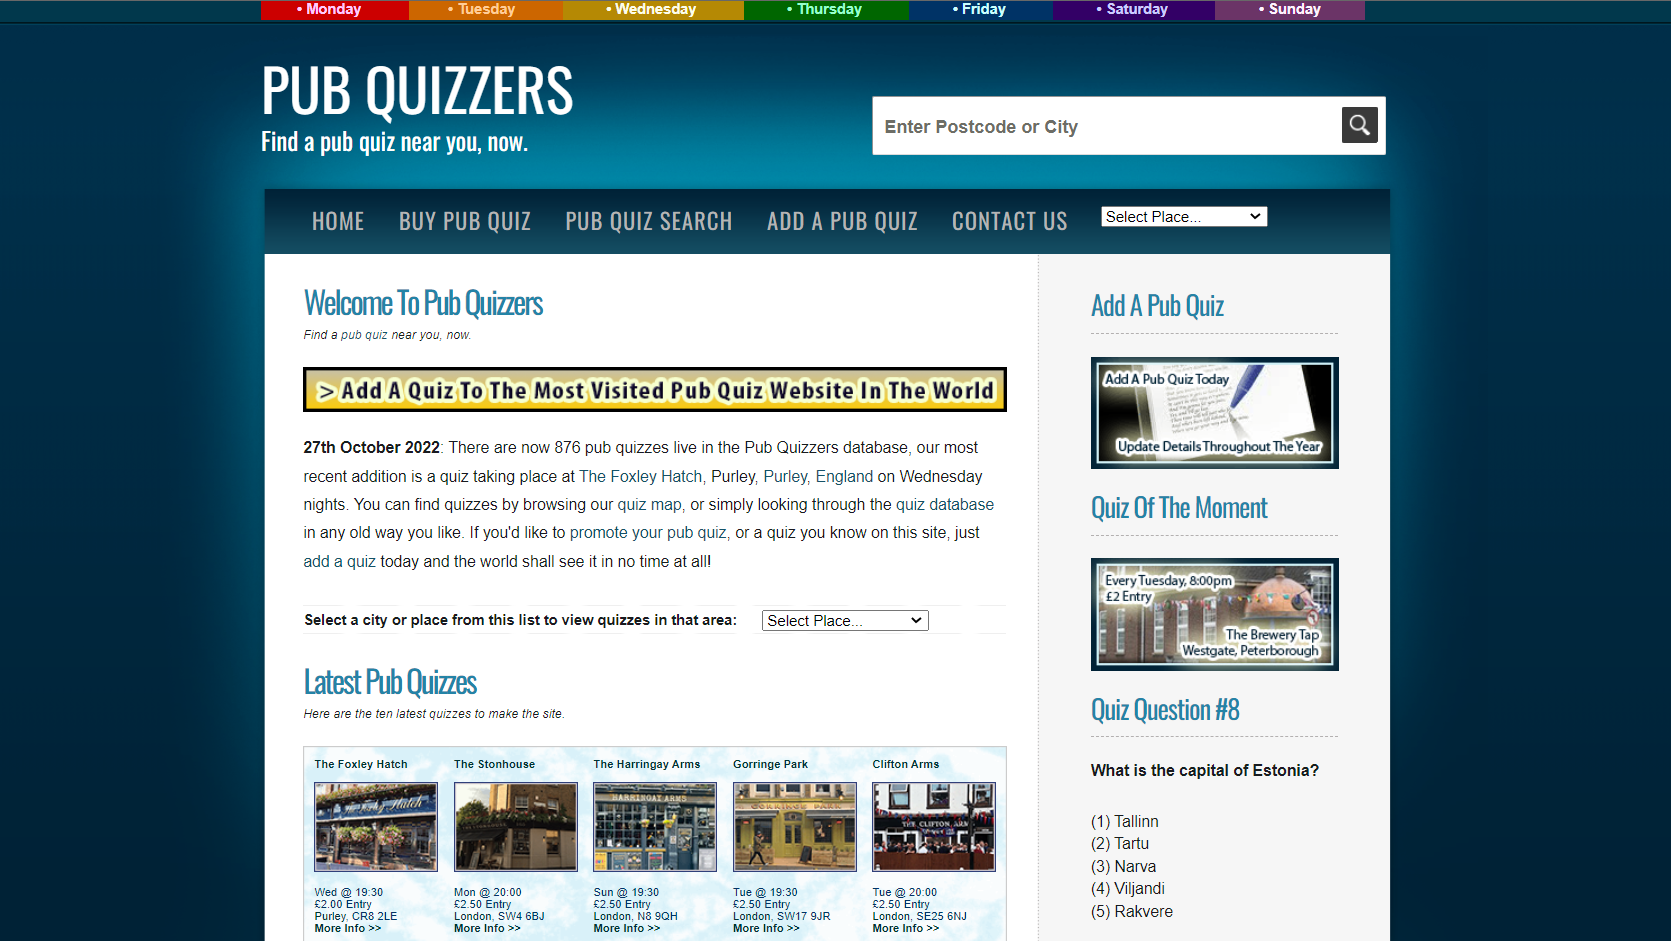
\includegraphics[width=\textwidth]{slike/slicnoRjesenje.PNG} 
			\caption{Primjer sličnog rješenja}
			\label{fig:slicnoRjesenje}
		\end{figure}

		
		
	
	\chapter{Specifikacija programske potpore}
		
	\section{Funkcionalni zahtjevi}
			
			\textbf{\textit{dio 1. revizije}}\\
			
			\textit{Navesti \textbf{dionike} koji imaju \textbf{interes u ovom sustavu} ili  \textbf{su nositelji odgovornosti}. To su prije svega korisnici, ali i administratori sustava, naručitelji, razvojni tim.}\\
				
			\textit{Navesti \textbf{aktore} koji izravno \textbf{koriste} ili \textbf{komuniciraju sa sustavom}. Oni mogu imati inicijatorsku ulogu, tj. započinju određene procese u sustavu ili samo sudioničku ulogu, tj. obavljaju određeni posao. Za svakog aktora navesti funkcionalne zahtjeve koji se na njega odnose.}\\
			
			
			\noindent \textbf{Dionici:}
			
			\begin{packed_enum}
				
				\item Naručitelj
				\item Korisnik aplikacije
				\begin{packed_enum}
					\item Igrač kviza
					\item Sastavljač kviza
				\end{packed_enum}				
				\item Administratori
				\item Razvojni tim
				
			\end{packed_enum}
			
			\noindent \textbf{Aktori i njihovi funkcionalni zahtjevi:}
			
			
			\begin{packed_enum}
				\item  \underbar{Neregistrirani/neprijavljeni korisnik (inicijator) može:}
				
				\begin{packed_enum}
					
					\item registrirati se u sustav kao igrač, sastavljač ili oboje istovremeno
					\item pregledati osnovne informacije o događaju (pub kvizu)
					
				\end{packed_enum}
			
				\item  \underbar{Igrač kviza (inicijator) može:}
				
				\begin{packed_enum}
					
					\item prijaviti se u sustav
					\item vidjeti sve objavljene događaje na pregledu "Svi pub kvizovi"
					\item vidjeti događaje na koje je prijavljen na pregledu "Moji pub kvizovi"
					\item pronaći ekipu za kviz
					\item napustiti svoju ekipu
					\item prijaviti svoju ekipu na kviz					
					\item pregledati svoj profil
					\item uređivati svoj profil
					\item pregledati profil sastavljača					 
					\item pretraživati i filtrirati događaje
					\item vidjeti statističke podatke				
							
				\end{packed_enum}
			
				\item  \underbar{Sastavljač kviza (inicijator) može:}
				
				\begin{packed_enum}
					
					\item prijaviti se u sustav
					\item objaviti novi događaj (pub kviz)
					\item vidjeti sve objavljene događaje na pregledu "Svi pub kvizovi"
					\item vidjeti svoje objavljene događaje na pregledu "Moji pub kvizovi"				
					\item pregledati svoj profil
					\item uređivati svoj profil							 
					\item pretraživati i filtrirati događaje
					\item vidjeti statističke podatke	
					
				\end{packed_enum}
			
				\item  \underbar{Administrator (inicijator) može:}
				
				\begin{packed_enum}
					
					\item sve isto što mogu i ostali korisnici sustava
					\item blokirati korisnike koji krše pravila sustava 
					\item odobriti ili zabraniti objavu koju je kreirao sastavljač
					\item brisati objavljene događaje
					\item davati administratorska prava drugim korisnicima
					
				\end{packed_enum}
			
				\item  \underbar{Baza podataka (sudionik) može:}
				
				\begin{packed_enum}
					
					\item pohranjivati sve podatke o korisnicima i njihovim ovlastima
					\item pohranjivati sve podatke o događajima (kvizovima)
					
				\end{packed_enum}
			\end{packed_enum}
			
			\eject 
			
			
				
			\subsection{Obrasci uporabe}
				
				\textbf{\textit{dio 1. revizije}}
				
				\subsubsection{Opis obrazaca uporabe}
					\textit{Funkcionalne zahtjeve razraditi u obliku obrazaca uporabe. Svaki obrazac je potrebno razraditi prema donjem predlošku. Ukoliko u nekom koraku može doći do odstupanja, potrebno je to odstupanje opisati i po mogućnosti ponuditi rješenje kojim bi se tijek obrasca vratio na osnovni tijek.}\\
					

				\noindent \underbar{\textbf{UC$$01$$ - $$Pregled naslovnice$$}}
				\begin{packed_item}
					
					\item \textbf{Glavni sudionik:} Neregistrirani korisnik, registrirani korisnik
					\item  \textbf{Cilj:} Pregledati naslovnicu aplikacije
					\item  \textbf{Sudionici:} Baza podataka
					\item  \textbf{Preduvjet:} Korisnik nije prijavljen u sustav
					\item  \textbf{Opis osnovnog tijeka:}
					
					\item[] \begin{packed_enum}
						
						\item Korisnik pregledava opis i sve objavljene događaje na naslovnici
						
					\end{packed_enum}
					
					\item  \textbf{Opis mogućih odstupanja:}
					
					\item[] \begin{packed_item}
						
						\item[1.a] Ne postoji ni jedan objavljeni događaj
						\item[] \begin{packed_enum}
							
							\item Korisniku se prikazuje samo opis aplikacije
							
						\end{packed_enum}
					\end{packed_item}
				\end{packed_item}
				
				\noindent \underbar{\textbf{UC$$02$$ - $$Registracija$$}}
				\begin{packed_item}
					
					\item \textbf{Glavni sudionik:} Neregistrirani korisnik
					\item  \textbf{Cilj:} Stvoriti korisnički račun za pristup sustavu
					\item  \textbf{Sudionici:} Baza podataka
					\item  \textbf{Preduvjet:} -
					\item  \textbf{Opis osnovnog tijeka:}
					
					\item[] \begin{packed_enum}
						
						\item Korisnik odabire opciju za registraciju
						\item Korisnik unosi tražene podatke i potvrđuje unos
						\item Podaci se spremaju u bazu podataka
						\item Korisnika se preusmjerava na početnu stranicu
						
					\end{packed_enum}
					
					\item  \textbf{Opis mogućih odstupanja:}
					
					\item[] \begin{packed_item}
						
						\item[2.a] Korisnik unosi neispravne podatke (zauzeti ili neispravni e-mail ili nadimak, unos podataka u nedopuštenom formatu)
						\item[] \begin{packed_enum}
							
							\item Sustav upozorava korisnika na neispravnost unesenih podataka i vraća ga na stranicu za registraciju.
							\item Korisnik mijenja podatke ili odustaje od registracije
							
						\end{packed_enum}
					\end{packed_item}
				\end{packed_item}
				
				\noindent \underbar{\textbf{UC$$03$$ - $$Prijava u sustav$$}}
				\begin{packed_item}
					
					\item \textbf{Glavni sudionik:} Registrirani korisnik
					\item  \textbf{Cilj:} Pristupiti korisničkom sučelju
					\item  \textbf{Sudionici:} Baza podataka
					\item  \textbf{Preduvjet:} Korisnik je registriran u sustav
					\item  \textbf{Opis osnovnog tijeka:}
					
					\item[] \begin{packed_enum}
						
						\item Korisnik unosi nadimak i lozinku te potvrđuje unos
						\item Sustav provjerava ispravnost unesenih podataka
						\item Korisnik dobiva pristup korisničkom sučelju
					\end{packed_enum}
					
					\item  \textbf{Opis mogućih odstupanja:}
					
					\item[] \begin{packed_item}
						
						\item[2.a] Uneseni su neispravni nadimak i/ili lozinka 
						\item[] \begin{packed_enum}
							
							\item Sustav obavještava korisnika da su uneseni pogrešni podaci i vraća ga na stranicu za prijavu			
						\end{packed_enum}			
					\end{packed_item}
				\end{packed_item}
				
				
				\noindent \underbar{\textbf{UC$$04$$ - $$Pregled podataka korisničkog profila$$}}
				\begin{packed_item}
					
					\item \textbf{Glavni sudionik:} Registrirani korisnik
					\item  \textbf{Cilj:} Pregledati podatke korisničkog profila
					\item  \textbf{Sudionici:} Baza podataka
					\item  \textbf{Preduvjet:} Korisnik je prijavljen u sustav
					\item  \textbf{Opis osnovnog tijeka:}
					
					\item[] \begin{packed_enum}
						
						\item Korisnik odabire opciju „Moj profil"
						\item Korisnik pregledava podatke profila
					\end{packed_enum}
					
				\end{packed_item}
				
				
				\noindent \underbar{\textbf{UC$$05$$ - $$Uređivanje podataka korisničkog profila$$}}
				\begin{packed_item}
					
					\item \textbf{Glavni sudionik:} Registrirani korisnik
					\item  \textbf{Cilj:} Urediti podatke korisničkog profila
					\item  \textbf{Sudionici:} Baza podataka
					\item  \textbf{Preduvjet:} Korisnik je prijavljen u sustav
					\item  \textbf{Opis osnovnog tijeka:}
					
					\item[] \begin{packed_enum}
						
						\item Korisnik odabire opciju „Moj profil“
						\item Korisnik odabire opciju za promjenu podataka
						\item Korisnik mijenja odabrane podatke
						\item Korisnik sprema promjene
						\item Baza podataka se ažurira
					\end{packed_enum}
					
					\item  \textbf{Opis mogućih odstupanja:}
					
					\item[] \begin{packed_item}
						
						\item[4.a] Korisnik ne spremi promjene
						\item[] \begin{packed_enum}
							
							\item Promjene se odbacuju
							
						\end{packed_enum}
						
					\end{packed_item}
				\end{packed_item}
				
				
				\noindent \underbar{\textbf{UC$$06$$ - $$Kreiranje nadolazećih događaja$$}}
				\begin{packed_item}
					
					\item \textbf{Glavni sudionik:} Registrirani korisnik (Sastavljač kviza)
					\item  \textbf{Cilj:} Kreirati nove događaje
					\item  \textbf{Sudionici:} Baza podataka
					\item  \textbf{Preduvjet:} Korisnik je prijavljen u sustav
					\item  \textbf{Opis osnovnog tijeka:}
					
					\item[] \begin{packed_enum}
						
						\item Korisnik odabire opciju za kreiranje novog događaja
						\item Korisnik popunjava potrebne podatke
						\item Korisnik sprema promjene
						\item Podaci se spremaju u bazu podataka
						\item Novi kviz čeka odobrenje administratora
					\end{packed_enum}
					
					\item  \textbf{Opis mogućih odstupanja:}
					
					\item[] \begin{packed_item}
						
						\item[3.a] Korisnik je već kreirao događaj u isto vrijeme
						\item[] \begin{packed_enum}
							
							\item Sustav vraća poruku o neispravno unesenom podatku
							\item Korisnik unosi ispravno vrijeme ili odustaje od kreiranja događaja
							
						\end{packed_enum}
						
					\end{packed_item}
				\end{packed_item}
				
				
				\noindent \underbar{\textbf{UC$$07$$ - $$Odobravanje kreiranih događaja$$}}
				\begin{packed_item}
					
					\item \textbf{Glavni sudionik:} Administrator
					\item  \textbf{Cilj:} Odobriti nove događaje
					\item  \textbf{Sudionici:} Baza podataka
					\item  \textbf{Preduvjet:} Administrator je prijavljen u sustav
					\item  \textbf{Opis osnovnog tijeka:}
					
					\item[] \begin{packed_enum}
						
						\item Administratoru je dostupan popis novih događaja koji čekaju odobrenje
						\item Administrator odabire događaj i odobrava ga
						\item Baza podataka se ažurira
						\item Odobreni događaj se objavljuje
					\end{packed_enum}
				\end{packed_item}
				
				
				\noindent \underbar{\textbf{UC$$08$$ - $$Zabrana kreiranih događaja$$}}
				\begin{packed_item}
					
					\item \textbf{Glavni sudionik:} Administrator
					\item  \textbf{Cilj:} Zabraniti nove događaje
					\item  \textbf{Sudionici:} Baza podataka
					\item  \textbf{Preduvjet:} Administrator je prijavljen u sustav
					\item  \textbf{Opis osnovnog tijeka:}
					
					\item[] \begin{packed_enum}
						
						\item Administratoru je dostupan popis novih događaja koji čekaju odobrenje
						\item Administrator odabire događaj i zabranjuje ga
						\item Događaj se briše iz baze podataka
					\end{packed_enum}
					
				\end{packed_item}			
				
				
				\noindent \underbar{\textbf{UC$$09$$ - $$Pregled svih objavljenih događaja$$}}
				\begin{packed_item}
					
					\item \textbf{Glavni sudionik:} Registrirani korisnik
					\item  \textbf{Cilj:} Pregledati sve događaje koji su objavljeni
					\item  \textbf{Sudionici:} Baza podataka
					\item  \textbf{Preduvjet:} Korisnik je prijavljen u sustav
					\item  \textbf{Opis osnovnog tijeka:}
					
					\item[] \begin{packed_enum}
						
						\item Korisnik odabire opciju „Svi pub kvizovi“
						\item Korisniku se prikazuju svi objavljeni događaji
						
					\end{packed_enum}
					
					\item  \textbf{Opis mogućih odstupanja:}
					
					\item[] \begin{packed_item}
						
						\item[2.a] Ne postoji ni jedan objavljeni događaj
						\item[] \begin{packed_enum}
							
							\item Korisniku se prikazuje odgovarajuća poruka
							
						\end{packed_enum}
						
					\end{packed_item}
				\end{packed_item}
				
				
				\noindent \underbar{\textbf{UC$$10$$ - $$Pregled svojih objavljenih događaja$$}}
				\begin{packed_item}
					
					\item \textbf{Glavni sudionik:} Registrirani korisnik (Sastavljač kviza)
					\item  \textbf{Cilj:} Pregledati svoje objavljene događaje
					\item  \textbf{Sudionici:} Baza podataka
					\item  \textbf{Preduvjet:} Korisnik je prijavljen u sustav
					\item  \textbf{Opis osnovnog tijeka:}
					
					\item[] \begin{packed_enum}
						
						\item Korisnik odabire opciju „Moji pub kvizovi“
						\item Korisniku se prikazuju njegovi objavljeni događaji
					\end{packed_enum}
					
					\item  \textbf{Opis mogućih odstupanja:}
					
					\item[] \begin{packed_item}
						
						\item[2.a] Ne postoji ni jedan objavljeni događaj koji je korisnik kreirao
						\item[] \begin{packed_enum}
							
							\item Korisniku se prikazuje odgovarajuća poruka
							
						\end{packed_enum}
						
					\end{packed_item}
				\end{packed_item}
				
				
				\noindent \underbar{\textbf{UC$$11$$ - $$Pregled prijava za objavljene događaje$$}}
				\begin{packed_item}
					
					\item \textbf{Glavni sudionik:} Registrirani korisnik (Igrač kviza)
					\item  \textbf{Cilj:} Pregledati događaje na koje je korisnik prijavljen
					\item  \textbf{Sudionici:} Baza podataka
					\item  \textbf{Preduvjet:} Korisnik je prijavljen u sustav
					\item  \textbf{Opis osnovnog tijeka:}
					
					\item[] \begin{packed_enum}
						
						\item Korisnik odabire opciju "Moji pub kvizovi"
						\item Korisniku se prikazuju svi događaji na koje je prijavljena njegova ekipa
						
					\end{packed_enum}
					
					\item  \textbf{Opis mogućih odstupanja:}
					
					\item[] \begin{packed_item}
						
						\item[2.a] Korisnikova ekipa nije prijavljena ni na jedan događaj
						\item[] \begin{packed_enum}
							
							\item Korisniku se prikazuje odgovarajuća poruka
							
						\end{packed_enum}
						
					\end{packed_item}
				\end{packed_item}
				
				
				\noindent \underbar{\textbf{UC$$12$$ - $$Pregled detalja objavljenog događaja$$}}
				\begin{packed_item}
					
					\item \textbf{Glavni sudionik:} Registrirani korisnik
					\item  \textbf{Cilj:} Pregledati detalje o objavljenom događaju
					\item  \textbf{Sudionici:} Baza podataka
					\item  \textbf{Preduvjet:} Korisnik je prijavljen u sustav
					\item  \textbf{Opis osnovnog tijeka:}
					
					\item[] \begin{packed_enum}
						
						\item Korisnik odabire opciju "Svi pub kvizovi"
						\item Korisnik odabire pregled detalja određenog događaja
						\item Korisniku se prikazuju detalji odabranog događaja
						
					\end{packed_enum}
					
					\item  \textbf{Opis mogućih odstupanja:}
					
					\item[] \begin{packed_item}
						
						\item[1.a] Ne postoji ni jedan objavljeni događaj
						\item[] \begin{packed_enum}
							
							\item Korisniku se prikazuje odgovarajuća poruka
							
						\end{packed_enum}
						
					\end{packed_item}
				\end{packed_item}
				
				
				\noindent \underbar{\textbf{UC$$13$$ - $$Pretraživanje objavljenih događaja$$}}
				\begin{packed_item}
					
					\item \textbf{Glavni sudionik:} Registrirani korisnik
					\item  \textbf{Cilj:} Na lakši način pronaći željeni događaj
					\item  \textbf{Sudionici:} Baza podataka
					\item  \textbf{Preduvjet:} Korisnik je prijavljen u sustav
					\item  \textbf{Opis osnovnog tijeka:}
					
					\item[] \begin{packed_enum}
						
						\item Korisnik na pregledu objavljenih događaja unosi željene podatke za pretraživanje te potvrđuje unos
						\item Korisniku se prikazuju događaji koji odgovaraju podacima unesenim za pretragu
						
					\end{packed_enum}
					
					\item  \textbf{Opis mogućih odstupanja:}
					
					\item[] \begin{packed_item}
						
						\item[2.a] Ni jedan događaj ne odgovara pretraživanim podacima
						\item[] \begin{packed_enum}
							
							\item Korisniku se prikazuje odgovarajuća poruka
							
						\end{packed_enum}
						
					\end{packed_item}
				\end{packed_item}
				
				
				\noindent \underbar{\textbf{UC$$14$$ - $$Filtriranje objavljenih događaja$$}}
				\begin{packed_item}
					
					\item \textbf{Glavni sudionik:} Registrirani korisnik
					\item  \textbf{Cilj:} Pronaći događaj koji najviše odgovara korisniku
					\item  \textbf{Sudionici:} Baza podataka
					\item  \textbf{Preduvjet:} Korisnik je prijavljen u sustav
					\item  \textbf{Opis osnovnog tijeka:}
					
					\item[] \begin{packed_enum}
						
						\item  Korisnik na pregledu objavljenih događaja odabire željene filtre za pretraživanje specifičnih događaja te potvrđuje unos
						\item Korisniku se prikazuju događaji koji odgovaraju odabranim filtrima
						
					\end{packed_enum}
					
					\item  \textbf{Opis mogućih odstupanja:}
					
					\item[] \begin{packed_item}
						
						\item[2.a] Ni jedan događaj ne odgovara filtriranim podacima
						\item[] \begin{packed_enum}
							
							\item Korisniku se prikazuje odgovarajuća poruka
							
						\end{packed_enum}
						
					\end{packed_item}
				\end{packed_item}
				
				
				\noindent \underbar{\textbf{UC$$15$$ - $$Pronalazak ekipe za kviz$$}}
				\begin{packed_item}
					
					\item \textbf{Glavni sudionik:} Registrirani korisnik (Igrač kviza)
					\item  \textbf{Cilj:} Pronaći ekipu za sudjelovanje na događajima
					\item  \textbf{Sudionici:} Baza podataka
					\item  \textbf{Preduvjet:} Korisnik je prijavljen u sustav
					\item  \textbf{Opis osnovnog tijeka:}
					
					\item[] \begin{packed_enum}
						
						\item Korisnik odabire opciju za pronalazak ekipe
						\item Sustav pronalazi ekipu najbolje odgovara korisniku
						\item Sustav šalje obavijest korisniku o ekipi u koju je dodan
						\item Sustav šalje obavijest  o korisniku članovima ekipe u koju je dodan 
						
					\end{packed_enum}
					
					\item  \textbf{Opis mogućih odstupanja:}
					
					\item[] \begin{packed_item}
						
						\item[2.a] U sustavu ne postoji ni jedna ekipa
						\item[] \begin{packed_enum}
							
							\item Korisniku se prikazuje odgovarajuća poruka
							
						\end{packed_enum}
						
						\item[2.b] Sve ekipe u sustavu imaju maksimalan broj članova
						\item[] \begin{packed_enum}
							
							\item Korisniku se prikazuje odgovarajuća poruka
							
						\end{packed_enum}
						
					\end{packed_item}				
				\end{packed_item}
				
				
				\noindent \underbar{\textbf{UC$$16$$ - $$Pregled obavijesti o pronađenoj ekipi$$}}
				\begin{packed_item}
					
					\item \textbf{Glavni sudionik:} Registrirani korisnik (Igrač kviza)
					\item  \textbf{Cilj:} Pregledati obavijest o pronalasku ekipe
					\item  \textbf{Sudionici:} Baza podataka
					\item  \textbf{Preduvjet:} Korisnik je prijavljen u sustav, prethodno je odabrao opciju za pronalazak ekipe i dodan je u neku ekipu
					\item  \textbf{Opis osnovnog tijeka:}
					
					\item[] \begin{packed_enum}
						
						\item Korisnik odabire opciju za pregled obavijesti
						\item Korisnik pregledava obavijest o pronađenoj ekipi
						
					\end{packed_enum}
					
				\end{packed_item}
				
				
				\noindent \underbar{\textbf{UC$$17$$ - $$Pregled obavijesti o novom članu ekipe$$}}
				\begin{packed_item}
					
					\item \textbf{Glavni sudionik:} Registrirani korisnik (Igrač kviza)
					\item  \textbf{Cilj:} Pregledati obavijest o dodavanju novog člana u ekipu
					\item  \textbf{Sudionici:} Baza podataka
					\item  \textbf{Preduvjet:} Korisnik je prijavljen u sustav i pripada ekipi u koju je dodan neki novi član
					\item  \textbf{Opis osnovnog tijeka:}
					
					\item[] \begin{packed_enum}
						
						\item Korisnik odabire opciju za pregled obavijesti
						\item Korisnik pregledava obavijest o novom članu ekipe
						
					\end{packed_enum}
					
				\end{packed_item}
				
				
				\noindent \underbar{\textbf{UC$$18$$ - $$Napuštanje ekipe$$}}
				\begin{packed_item}
					
					\item \textbf{Glavni sudionik:} Registrirani korisnik (Igrač kviza)
					\item  \textbf{Cilj:} Napustiti trenutnu ekipu
					\item  \textbf{Sudionici:} Baza podataka
					\item  \textbf{Preduvjet:} Igrač je prijavljen u sustav i trenutno se nalazi u nekoj ekipi
					\item  \textbf{Opis osnovnog tijeka:}
					
					\item[] \begin{packed_enum}
						
						\item Korisnik odabire opciju ”Moj profil”
						\item Korisnik odabire opciju napuštanja trenutne ekipe
						\item Sustav izbacuje korisnika iz trenutne ekipe i šalje obavijest ostalim članovima da je korisnik napustio ekipu
						\item Baza podataka se ažurira
						
					\end{packed_enum}
					
					\item  \textbf{Opis mogućih odstupanja:}
					
					\item[] \begin{packed_item}
						
						\item[3.a] Korisnik je prije odabira opcije napuštanja ekipe bio jedini njezin član
						\item[] \begin{packed_enum}
							
							\item Sustav nikome ne šalje obavijest o napuštanju
							
						\end{packed_enum}
						
					\end{packed_item}
				\end{packed_item}
				
				
				\noindent \underbar{\textbf{UC$$19$$ - $$Pregled obavijesti o napuštanju člana ekipe$$}}
				\begin{packed_item}
					
					\item \textbf{Glavni sudionik:} Registrirani korisnik (Igrač  kviza)
					\item  \textbf{Cilj:} Pregledati obavijest o napuštanju člana ekipe
					\item  \textbf{Sudionici:} Baza podataka
					\item  \textbf{Preduvjet:} Korisnik je prijavljen u sustav
					\item  \textbf{Opis osnovnog tijeka:}
					
					\item[] \begin{packed_enum}
						
						\item Korisnik odabire opciju za pregled obavijesti
						\item Korisnik pregledava obavijest o napuštanju člana ekipe
					\end{packed_enum}
					
				\end{packed_item}
				
				
				\noindent \underbar{\textbf{UC$$20$$ - $$Prijava ekipe na događaj$$}}
				\begin{packed_item}
					
					\item \textbf{Glavni sudionik:} Registrirani korisnik (Igrač kviza)
					\item  \textbf{Cilj:} Prijaviti ekipu na događaj
					\item  \textbf{Sudionici:} Baza podataka
					\item  \textbf{Preduvjet:} Korisnik je prijavljen u sustav
					\item  \textbf{Opis osnovnog tijeka:}
					
					\item[] \begin{packed_enum}
						
						\item Korisnik pregledava sve objavljene događaje
						\item Korisnik odabire događaj na koji želi prijaviti ekipu
						\item Korisnik prijavljuje ekipu na događaj
						\item Baza podataka se ažurira
					\end{packed_enum}
					
					\item  \textbf{Opis mogućih odstupanja:}
					
					\item[] \begin{packed_item}
						
						\item[2.a] Ekipa je već prijavljena na neki događaj u isto vrijeme
						\item[] \begin{packed_enum}
							
							\item Korisniku se prikazuje odgovarajuća poruka i odbija se prijava ekipe za taj događaj
							
						\end{packed_enum}
						
					\end{packed_item}
					
				\end{packed_item}
				
				
				\noindent \underbar{\textbf{UC$$21$$ - $$Pregled obavijesti o prijavi na događaj$$}}
				\begin{packed_item}
					
					\item \textbf{Glavni sudionik:} Registrirani korisnik (Igrač kviza)
					\item  \textbf{Cilj:} Pregledati obavijest o prijavi na događaj
					\item  \textbf{Sudionici:} Baza podataka
					\item  \textbf{Preduvjet:} Korisnik je prijavljen u sustav
					\item  \textbf{Opis osnovnog tijeka:}
					
					\item[] \begin{packed_enum}
						
						\item Korisnik odabire opciju za pregled obavijesti
						\item Korisnik pregledava obavijest o prijavi na događaj zajedno s informacijama događaja
					\end{packed_enum}
					
				\end{packed_item}
				
				
				\noindent \underbar{\textbf{UC$$22$$ - $$Blokiranje korisnika$$}}
				\begin{packed_item}
					
					\item \textbf{Glavni sudionik:} Administrator
					\item  \textbf{Cilj:} Blokirati korisnika
					\item  \textbf{Sudionici:} Baza podataka
					\item  \textbf{Preduvjet:} Administrator je prijavljen u sustav
					\item  \textbf{Opis osnovnog tijeka:}
					
					\item[] \begin{packed_enum}
						
						\item Administrator pregledava listu svih korisnika
						\item Administrator odabire opciju blokiranja korisnika
						\item Administrator pronalazi željenog korisnika
						\item Administrator blokira korisnika
						\item Baza podataka se ažurira
					\end{packed_enum}
					
				\end{packed_item}
				
				
				\noindent \underbar{\textbf{UC$$23$$ - $$Brisanje objavljenih događaja$$}}
				\begin{packed_item}
					
					\item \textbf{Glavni sudionik:} Administrator
					\item  \textbf{Cilj:} Obrisati objavljeni događaj
					\item  \textbf{Sudionici:} Baza podataka
					\item  \textbf{Preduvjet:} Administrator je prijavljen u sustav
					\item  \textbf{Opis osnovnog tijeka:}
					
					\item[] \begin{packed_enum}
						
						\item Administrator pregledava sve objavljene događaje
						\item Administrator odabire opciju brisanja događaja
						\item Administrator odabire događaj koji želi obrisati
						\item Administrator briše događaj
						\item Baza podataka se ažurira
					\end{packed_enum}
					
					\item  \textbf{Opis mogućih odstupanja:}
					
					\item[] \begin{packed_item}
						
						\item[1.a] Ne postoji ni jedan objavljeni događaj
						\item[] \begin{packed_enum}
							
							\item Administratoru se prikazuje odgovarajuća poruka
							
						\end{packed_enum}
						
					\end{packed_item}
				\end{packed_item}
				
				
				\noindent \underbar{\textbf{UC$$24$$ - $$Dodjela administratorskih prava korisniku$$}}
				\begin{packed_item}
					
					\item \textbf{Glavni sudionik:} Administrator
					\item  \textbf{Cilj:} Dodijeliti administratorska prava korisniku
					\item  \textbf{Sudionici:} Baza podataka
					\item  \textbf{Preduvjet:} Administrator je prijavljen u sustav
					\item  \textbf{Opis osnovnog tijeka:}
					
					\item[] \begin{packed_enum}
						
						\item Administrator pregledava listu svih korisnika					
						\item Administrator bira korisnika kojem želi dodijeliti administratorska prava
						\item Administrator dodjeljuje administratorska prava korisniku
						\item Baza podataka se ažurira
					\end{packed_enum}
					
				\end{packed_item}
				
				
				\noindent \underbar{\textbf{UC$$25$$ - $$Pregled profila sastavljača$$}}
				\begin{packed_item}
					
					\item \textbf{Glavni sudionik:} Registrirani korisnik
					\item  \textbf{Cilj:} Pregledati podatke profila sastavljača
					\item  \textbf{Sudionici:} Baza podataka
					\item  \textbf{Preduvjet:} Korisnik je prijavljen u sustav
					\item  \textbf{Opis osnovnog tijeka:}
					
					\item[] \begin{packed_enum}
						
						\item Korisnik pregledava sve objavljene događaje
						\item Korisnik odabire željeni događaj
						\item Korisnik pregledava detalje o odabranom događaju
						\item Korisnik odabire poveznicu na profil sastavljača
						\item Korisnik pregledava podatke profila sastavljača
					\end{packed_enum}
					
					\item  \textbf{Opis mogućih odstupanja:}
					
					\item[] \begin{packed_item}
						
						\item[1.a] Ne postoji ni jedan objavljeni događaj
						\item[] \begin{packed_enum}
							
							\item Administratoru se prikazuje odgovarajuća poruka
							
						\end{packed_enum}
						
					\end{packed_item}
				\end{packed_item}
				
				
				\noindent \underbar{\textbf{UC$$26$$ - $$Pregled statistike$$}}
				\begin{packed_item}
					
					\item \textbf{Glavni sudionik:} Registrirani korisnik (Igrač kviza)
					\item  \textbf{Cilj:} Pregledati statistiku 
					\item  \textbf{Sudionici:} Baza podataka
					\item  \textbf{Preduvjet:} Korisnik je prijavljen u sustav
					\item  \textbf{Opis osnovnog tijeka:}
					
					\item[] \begin{packed_enum}
						
						\item Korisnik odabire pregled „Statistika“
						\item Korisnik pregledava prikazane statističke podatke
					\end{packed_enum}
					
					\item  \textbf{Opis mogućih odstupanja:}
					
					\item[] \begin{packed_item}
						
						\item[2.a] Ne postoje odgovarajući podaci za prikaz
						\item[] \begin{packed_enum}
							
							\item Korisniku se prikazuje odgovarajuća poruka
							
						\end{packed_enum}
						
					\end{packed_item}
				\end{packed_item}
				
				
				\noindent \underbar{\textbf{UC$$27$$ - $$Odjava iz sustava$$}}
				\begin{packed_item}
					
					\item \textbf{Glavni sudionik:} Registrirani korisnik
					\item  \textbf{Cilj:} Odjaviti se iz sustava
					\item  \textbf{Sudionici:} -
					\item  \textbf{Preduvjet:} Korisnik je prijavljen u sustav
					\item  \textbf{Opis osnovnog tijeka:}
					
					\item[] \begin{packed_enum}
						
						\item Korisnik odabire opciju za odjavu iz sustava
						\item Korisnika se preusmjerava na stranicu za prijavu
						
					\end{packed_enum}
					
				\end{packed_item}
				
			
			
				
					
				\subsubsection{Dijagrami obrazaca uporabe}
					
					\textit{Prikazati odnos aktora i obrazaca uporabe odgovarajućim UML dijagramom. Nije nužno nacrtati sve na jednom dijagramu. Modelirati po razinama apstrakcije i skupovima srodnih funkcionalnosti.}
				\eject		
				
			\subsection{Sekvencijski dijagrami}
				
				\textbf{\textit{dio 1. revizije}}\\
				
				\textit{Nacrtati sekvencijske dijagrame koji modeliraju najvažnije dijelove sustava (max. 4 dijagrama). Ukoliko postoji nedoumica oko odabira, razjasniti s asistentom. Uz svaki dijagram napisati detaljni opis dijagrama.}
				\eject
	
		\section{Ostali zahtjevi}
		
			\textbf{\textit{dio 1. revizije}}\\
		 
			 \textit{Nefunkcionalni zahtjevi i zahtjevi domene primjene dopunjuju funkcionalne zahtjeve. Oni opisuju \textbf{kako se sustav treba ponašati} i koja \textbf{ograničenja} treba poštivati (performanse, korisničko iskustvo, pouzdanost, standardi kvalitete, sigurnost...). Primjeri takvih zahtjeva u Vašem projektu mogu biti: podržani jezici korisničkog sučelja, vrijeme odziva, najveći mogući podržani broj korisnika, podržane web/mobilne platforme, razina zaštite (protokoli komunikacije, kriptiranje...)... Svaki takav zahtjev potrebno je navesti u jednoj ili dvije rečenice.}
			 
			 
			 
	
	\chapter{Arhitektura i dizajn sustava}

    \begin{figure}[!h]
		\centering
		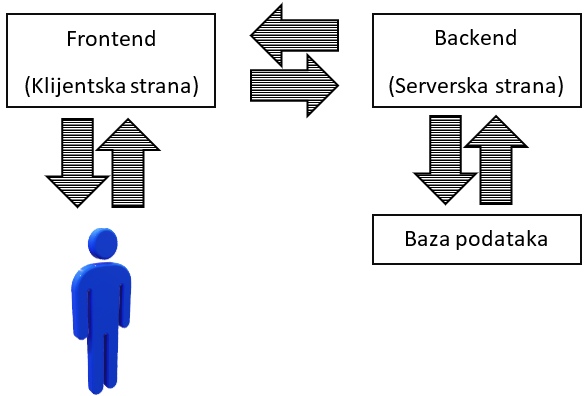
\includegraphics[width=13cm]{slike/arhitektura.PNG} 
		\caption{Arhitektura sustava}
		\label{fig:arhitektura}
	\end{figure}

	Korisnik aplikaciji pristupa putem web preglednika. Interakciju s aplikacijom ostvaruje preko korisničkog sučelja pomoću kojeg šalje zahtjeve web poslužitelju i prima odgovore.\\
Programski jezik pomoću kojeg je ostvaren backend web aplikacije je Java, a korišteni radni okvir je Spring Boot. Frontend aplikacije ostvaren je programskim jezikom JavaScript i bibliotekom React.js. Za razvojno okruženje odabran je Intellij IDEA. Spring Boot je radni okvir namijenjen stvaranju mikroservisa. Mikroservis je arhitektura koja omogućuje neovisan razvoj više različitih servisa od kojih svaki ima svoj proces.\\
Web aplikaciju čine tri osnovna dijela:
	\begin{itemize}
		\item 	\textbf{frontend}
		\item 	\textbf{backend}
		\item 	\textbf{baza podataka }		
	\end{itemize}
Frontend se sastoji od komponenata i logike. Istu komponentu je moguće koristiti za različite namjene (engl. reusability). React.js koristi virtualni DOM (engl. Document Object Model) čiji se sadržaj uspoređuje sa stvarnim DOM-om i na osnovu toga se provode promjene što za posljedicu ima poboljšanje performansi. Struktura ostvarena međusobnim povezivanjem različitih komponenti je stablo.\\
Backend se sastoji od: 
\begin{itemize}
		\item 	programskog sučelja za reprezentacijski prijenos stanja (REST API), odnosno Controller-a
		\item 	sloja poslovne logike (Service)
		\item 	sloja za pristup bazi podataka (Repository)		
	\end{itemize}
\textbf{Controller} izlaže funkcionalnost web aplikacije kao RESTful web usluge, tj. prima zahtjeve čiji su glavni dijelovi URI, metoda i HTTP zaglavlje, a korisniku šalje odgovor koji se sastoji od statusnog koda, tijela poruke i zaglavlja. U tijelu poruke se nalazi sadržaj kojeg korisnik konzumira nakon što je prikazan u web pregledniku. Komunikaciju sa slojem poslovne logike Controller ostvaruje pomoću umetanja ovisnosti (engl. dependency injection). Dependency injection je obrazac prema kojemu se u određeni objekt/funkciju umeće neki drugi objekt/funkcija na koji se prvobitno spomenuti objekt/funkcija oslanja.\\
\textbf{Service} omogućuje komunikaciju između slojeva Controller i Repository, zadužen je za provjeru ispravnosti podataka. Osim na sloju Service, provjera ispravnosti se obavlja na frontend-u i u bazi podataka. Komunikaciju sa slojem za pristup bazi podataka ostvaruje umetanjem ovisnosti.\\ 
\textbf{Repository} omogućuje komunikaciju s bazom podataka pomoću SQL-a. Objekti iz relacijske baze podataka pretvaraju se objekte programskog jezika Java korištenjem tehnike ORM.\\\\
		

				
		\section{Baza podataka}

		Baza podataka za aplikaciju implementirana je u obliku relacijske baze podataka, koja podatke sprema u obliku redaka ili n-torki i stupaca ili atributa koji zajedno tvore tablicu.  \\
Glavna komponenta baze je tablica Korisnik, koja se puni osobnim podacima unesenim pri registraciji u sustav.  Svakom novom korisniku dodjeljuje se primarni ključ, unikatan identifikacijski broj pomoću kojeg se korisnici u bazi podataka međusobno razlikuju. Budući da korisnik ima jednu ili više dodijeljenih uloga, koje su definirane u tablici Uloga, izrađena je veza između dvije tablice koja sadrži identifikacijske brojeve korisnika i odgovarajuće uloge. \\
Kako bi korisnik zaigrao na kvizu, potrebno je prvo pronaći ekipu kojoj odgovara svojim područjima znanja, zbog čega je izrađena tablica Ekipa koja sadrži minimalno jednoga, a maksimalno petero članova.  \\
Ako korisnik ima ulogu sastavljača, on kreira kviz s podacima i informacijama koji se spremaju u tablicu Kviz.  Svaki kviz ima svoj identifikacijski broj i unikatne atribute, vrijeme održavanja i ID sastavljača, jer jedan sastavljač ne može objaviti dva različita kviza koja se održavaju u isto vrijeme.  \\
Tablica Obavijest sadrži svoj identifikacijski broj, tekst obavijesti koji se prikazuje korisniku i ID korisnika kao strani ključ. \\

		
			\subsection{Opis tablica}
				
			
				\begin{longtblr} [
					label = none,
					entry = none
					] {
						width = \textwidth,
						colspec = {|X[8,l]|X[8, l]|X[16, l]|},
						rowhead = 1,
					}
					\hline \textbf{Korisnik} & \\ \hline[3pt]
					\SetCell{LightGreen}korisnik\_id & BIG INT & Identifikacijski broj korisnika, primarni ključ.\\ \hline
					ime & VARCHAR(100) & Ime korisnika. \\ \hline
					prezime & VARCHAR(100) & Prezime korisnika. \\ \hline
					email\_adresa(U) & VARCHAR(100) & E-mail adresa korisnika. \\ \hline
					lozinka & VARCHAR(50) & Lozinka koju korisnik osmisli pri registraciji. \\ \hline
					slika & VARBINARY & Profilna slika korisnika u aplikaciji, opcionalno. \\ \hline
					broj\_telefona & VARCHAR(50) & Broj telefona korisnika, opcionalno. \\ \hline
					podrucja\_znanja & VARCHAR(150) & Područja znanja igrača, koriste se pri odabiru ekipe. \\ \hline
					nadimak(U) & VARCHAR(50) & Nadimak koji si korisnik osmisli pri registraciji. \\ \hline
					prosj\_broj\_ekipa & INT & Prosječan broj ekipa koji sudjeluju u kvizovima nekog sastavljača, opcionalno. \\ \hline
					blokiran & BOOLEAN & Atribut koji daje informaciju o tome je li korisnik blokiran ili ne. \\ \hline
					\SetCell{LightBlue}ekipa\_id & BIG INT & Identifikacijski broj ekipe kojoj korisnik pripada, opcionalno. \\ \hline
				\end{longtblr}

				\begin{longtblr}[
					label = none,
					entry = none
				]{
					width = \textwidth,
					colspec = {|X[8,l]|X[8, l]|X[16, l]|},
					rowhead = 1,
                         		}
				\hline \textbf{Uloga} & \\ \hline[3pt]
				\SetCell{LightGreen} uloga\_id & BIG INT & Identifikacijski broj uloge. \\ \hline
				uloga\_ime & VARCHAR(50) & Ime uloge. \\ \hline
				\end{longtblr}



			
				\begin{longtblr}[
					label = none, 
					entry = none
					]{
						width = \textwidth,
						colspec = {|X[8,l]|X[8, l]|X[16, l]|},
						rowhead = 1,
					}
					\hline \textbf{korisnik\_uloga} & \\ \hline[3pt]
					\SetCell{LightBlue} uloga\_id & BIG INT & Identifikacijski broj uloge, strani ključ s referencom na ulogu.\\ \hline
					\SetCell{LightBlue} korisnik\_id & BIG INT & Identifikacijski broj korisnika, strani ključ s referencom na korisnika. \\ \hline
				\end{longtblr}
			
				\begin{longtblr} [
					label = none, 
					entry = none
					]{
						width = \textwidth,
						colspec = {|X[8,l]|X[8, l]|X[16, l]|},
						rowhead = 1,
					}
					\hline \textbf{Ekipa} & \\ \hline[3pt]
					\SetCell{LightGreen} ekipa\_id & BIG INT & Identifikacijski broj ekipe, primarni ključ. \\ \hline
					broj\_clanova & INT & Broj članova ekipe, ne smije biti manji od 1 ni veći od 5. \\ \hline
					naziv\_ekipe(U) & VARCHAR(50) & Ime ekipe. \\ \hline
				\end{longtblr}
			
			\begin{longtblr} [
				label = none,
				entry = none
				]{
					width = \textwidth,
					colspec = {|X[8,l]|X[8, l]|X[16, l]|},
					rowhead = 1,
				}
			\hline \textbf{Kviz} & \\ \hline[3pt]
			\SetCell{LightGreen} kviz\_id & BIG INT & Identifikacijski broj kviza, primarni ključ. \\ \hline
			kratki\_opis & VARCHAR(200) & Sažeti tekst o sadržaju kviza. \\ \hline
			ime\_kafica & VARCHAR(50) & Ime kafića u kojem se kviz održava. \\ \hline
			vrijeme\_odrzavanja (U) & TIMESTAMP & Vrijeme održavanja kviza, unikatan atribut zajedno s identifikacijskim brojem sastavljača. \\ \hline
			lokacija & GEOGRAPHY & Lokacija mjesta održavanja. \\ \hline
			maks\_broj\_ekipa & INT & Maksimalni broj ekipa koje sudjeluju na kvizu. \\ \hline
			kotizacija & FLOAT & Kotizacija za sudjelovanje na kvizu. \\ \hline
			nagrade & VARCHAR(100) & Popis nagrada na visoko plasirane ekipe. \\ \hline
			vrsta & VARCHAR(50) & Vrsta kviza (povijest, sport, ..). \\ \hline
			naziv\_kviza (U) & VARCHAR(50) & Unikatan naziv kviza. \\ \hline
			aktivan & BOOLEAN & Predstavlja je li kviz trenutno aktivan ili ne. \\ \hline
			\SetCell{LightBlue} korisnik\_id & BIG INT & Identifikacijski broj sastavljača, strani ključ s referencom na korisnika. \\ \hline
			\end{longtblr}

			

			\begin{longtblr}[
				label = none,
				entry = none
			]{
				width = \textwidth,
				colspec = {|X[8,l]|X[8, l]|X[16, l]|},
				rowhead = 1,
			}
			\hline \textbf{sudjeluje\_u} & \\ \hline[3pt]
			\SetCell{LightBlue} ekipa\_id & BIG INT & Identifikacijski broj ekipe, strani ključ s referencom na ekipu. \\ \hline
			\SetCell{LightBlue} kviz\_id & BIG INT & Identifikacijski broj kviza na kojem sudjeluje ekipa, strani ključ. \\ \hline
			\end{longtblr}

			\begin{longtblr} [
				label = none,
				entry = none
			]{
				width = \textwidth,
				colspec = {|X[8,l]|X[8, l]|X[16, l]|},
				rowhead = 1,
			}
			\hline \textbf{Obavijest}& \\ \hline[3pt]
			\SetCell{LightGreen} obavijest\_id & BIG INT & Identifikacijski broj obavijesti, primarni ključ. \\ \hline
			tekst & VARCHAR(300) & Tekst obavijesti. \\ \hline
			\SetCell{LightBlue} korisnik\_id & BIG INT & Identifikacijski broj korisnika koji je primio obavijest. \\ \hline
			\end{longtblr}
			
			
				
				
			
			\subsection{Dijagram baze podataka}
			 \begin{figure}[!h]
			\centering
			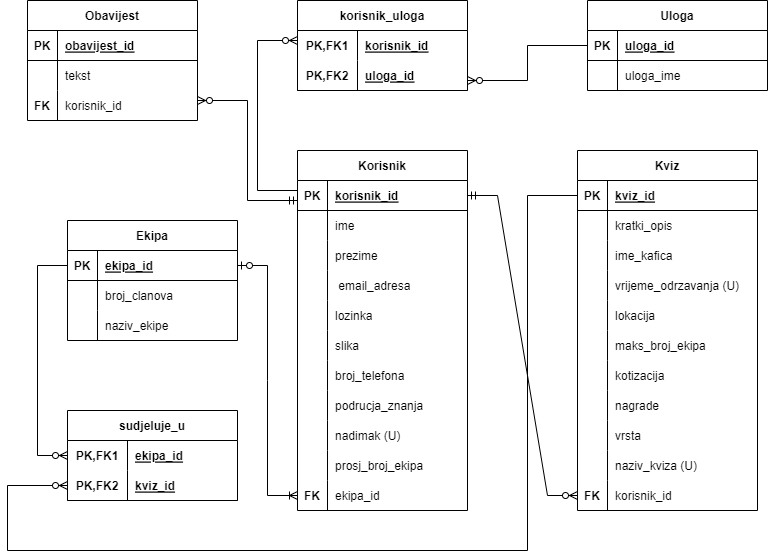
\includegraphics[width=15cm]{slike/final.png} 
			\caption{ER dijagram}
			\label{fig:arhitektura}
	\end{figure}
			
			\eject
			
			
		\section{Dijagram razreda}
		
			\begin{figure}[H]
				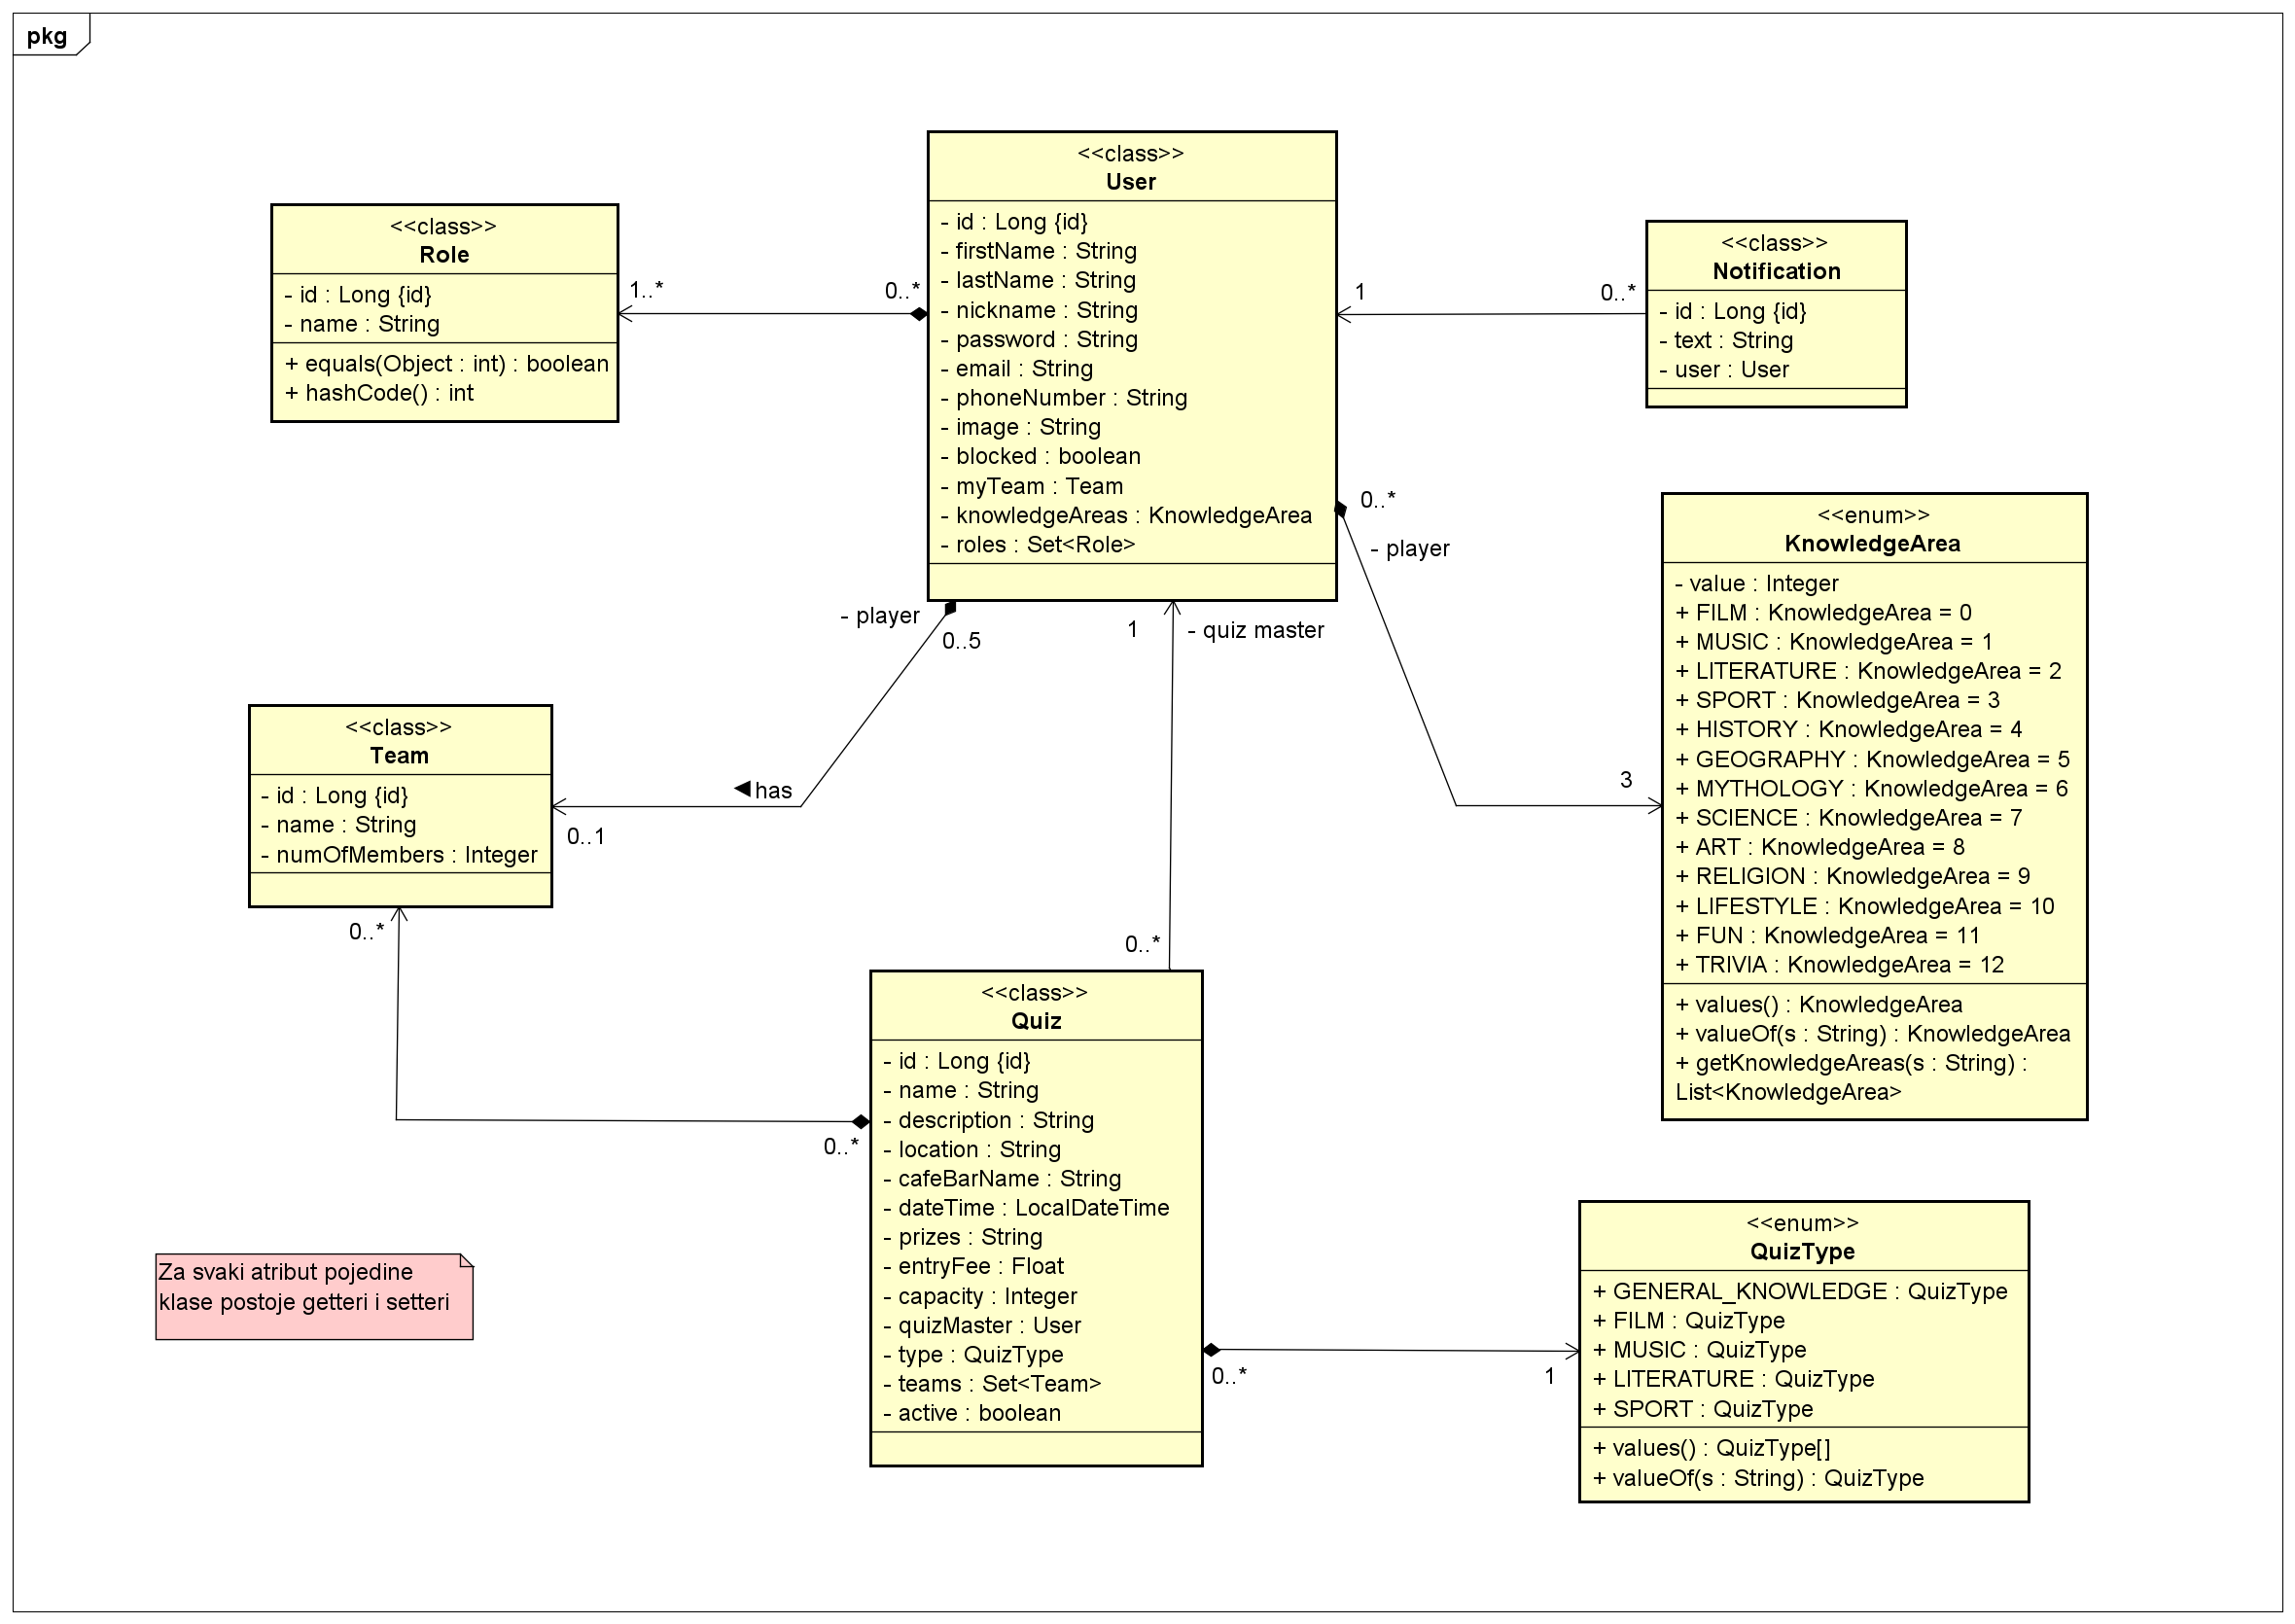
\includegraphics[width=\textwidth]{dijagrami/classDiagram1.PNG} 
				\caption{Dijagram razreda, dio Modeli}
				\label{fig:classDiagram1}
			\end{figure}
		
			Na slici 4.3 prikazan je dijagram razreda koji prikazuje razrede u objektno orijentiranom sustavu, njihove atribute i metode te međusobnu povezanost. Model razreda preslikava se u bazu podataka prema načelu ORM-a. Razred User predstavlja registriranog korisnika aplikacije koji može imati jednu ili više uloga opisane razredom Role. Korisnik prima obavijesti predstavljene razredom Notification, a kao igrač može pripadati najviše jednoj ekipi koja je opisana razredom Team. Također, korisnik koji je igrač izabire točno tri područja znanja koja su u aplikaciji ostvarena kao enumeracija KnowledgeArea. Korisnik koji je sastavljač može kreirati neograničen broj kvizova opisanih razredom Quiz, a svaki je kviz točno jedne vrste predstavljene enumeracijom QuizType te na jednom kvizu sudjeluje više ekipa, čiji je maksimalni broj određen atributom capacity razreda Quiz. 
			
			\begin{figure}[H]
				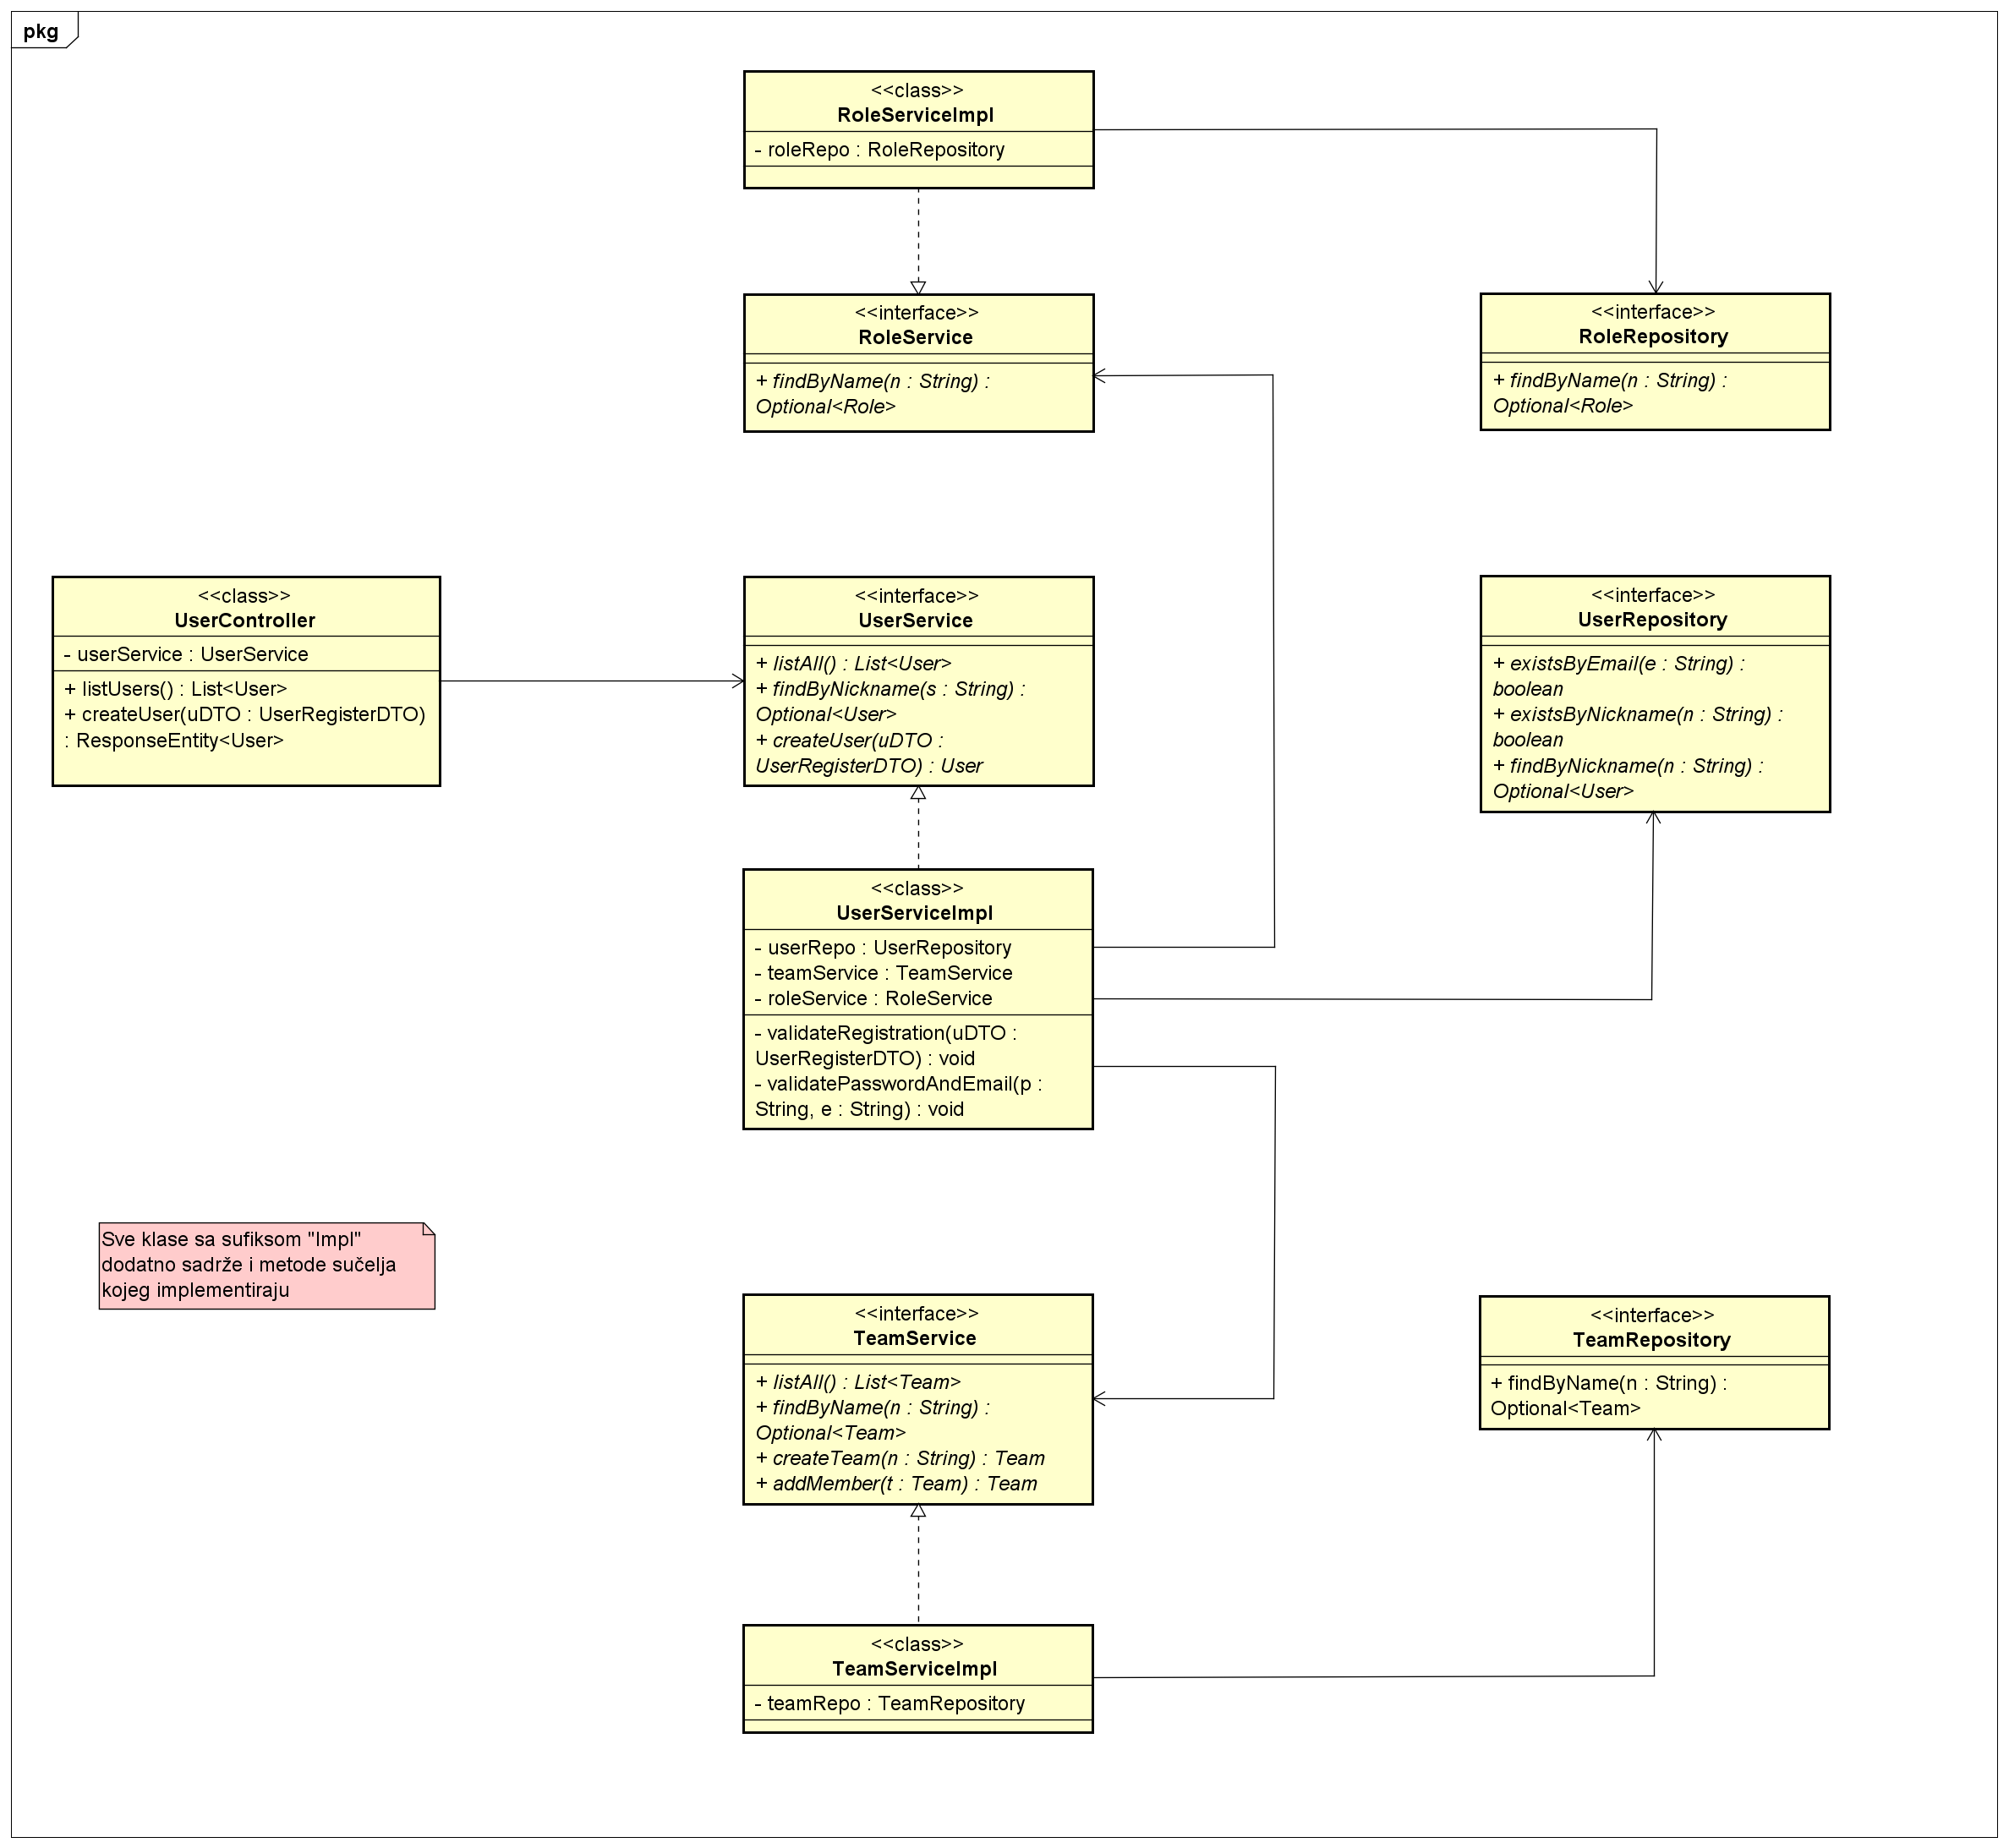
\includegraphics[width=\textwidth]{dijagrami/classDiagram2.PNG} 
				\caption{Dijagram razreda, kontroleri - servisi - repozitoriji}
				\label{fig:classDiagram2}
			\end{figure}
		
			Na slici 4.4 prikazan je dijagram razreda koji prikazuje organizaciju backenda aplikacije podijeljenu u tri sloja. Prvi sloj čini UserController koji prima zahtjeve i korisniku šalje odgovor te ostvaruje komunikaciju sa slojem poslovne logike u kojem se nalaze sučelja UserService, RoleService i TeamService s popisom potrebnih metoda te njihove pripadajuće implementacije - razredi UserServiceImpl, RoleServiceImpl i TeamServiceImpl. Svaki od navedenih razreda ostvaruje vezu sa svojim repozitorijem, a svaki repozitoriji predstavljen je sučeljem koje onda dodatno nasljeđuje sučelje JpaRepository\textless T, ID\textgreater{} radnog okvira Spring Boot za čiju se implementaciju on sam i pobrine.
			\newline\newline
	
			\textbf{\textit{dio 2. revizije}}\\			
			
			\textit{Prilikom druge predaje projekta dijagram razreda i opisi moraju odgovarati stvarnom stanju implementacije}
			
	
			
			\eject
		
		\section{Dijagram stanja}
			
			
			\textbf{\textit{dio 2. revizije}}\\
			
			\textit{Potrebno je priložiti dijagram stanja i opisati ga. Dovoljan je jedan dijagram stanja koji prikazuje \textbf{značajan dio funkcionalnosti} sustava. Na primjer, stanja korisničkog sučelja i tijek korištenja neke ključne funkcionalnosti jesu značajan dio sustava, a registracija i prijava nisu. }
			
			
			\eject 
		
		\section{Dijagram aktivnosti}
			
			\textbf{\textit{dio 2. revizije}}\\
			
			 \textit{Potrebno je priložiti dijagram aktivnosti s pripadajućim opisom. Dijagram aktivnosti treba prikazivati značajan dio sustava.}
			
			\eject
		\section{Dijagram komponenti}
		
			Dijagram komponenti je strukturni statički UML dijagram koji služi za vizualizaciju organizacije i međuovisnosti između implementacijskih komponenata i čini dio specifikacije arhitekture programske potpore. Za pristup sustavu koriste se dva sučelja. Preko sučelja I$\_$HTML$\_$CSS$\_$JS dohvaćaju se HTML, CSS i JS datoteke koje pripadaju frontend dijelu aplikacije. Komponenta Router na upit preko URL-a odlučuje koja će se datoteka poslužiti na sučelje. Frontend se sastoji od JavaScript datoteka koje su raspoređene po komponentama nazvanim prema stranicama aplikacije. Sve te datoteke ovise o React biblioteci iz koje dohvaćaju već gotove komponente poput formi i slično. Preko REST$\_$API sučelja pristupa se komponenti Controller koja poslužuje podatke iz backend dijela aplikacije. Repository je zadužen za dohvaćanje podataka iz tablica baze podataka pomoću SQL upita, a koristeći pritom SQL$\_$API sučelje. React-view komponenta preko dostupnih sučelja komunicira s aplikacijom te ovisno o korisnikovim akcijama osvježava prikaz i dohvaća nove podatke ili datoteke.
			
			\begin{figure}[H]
				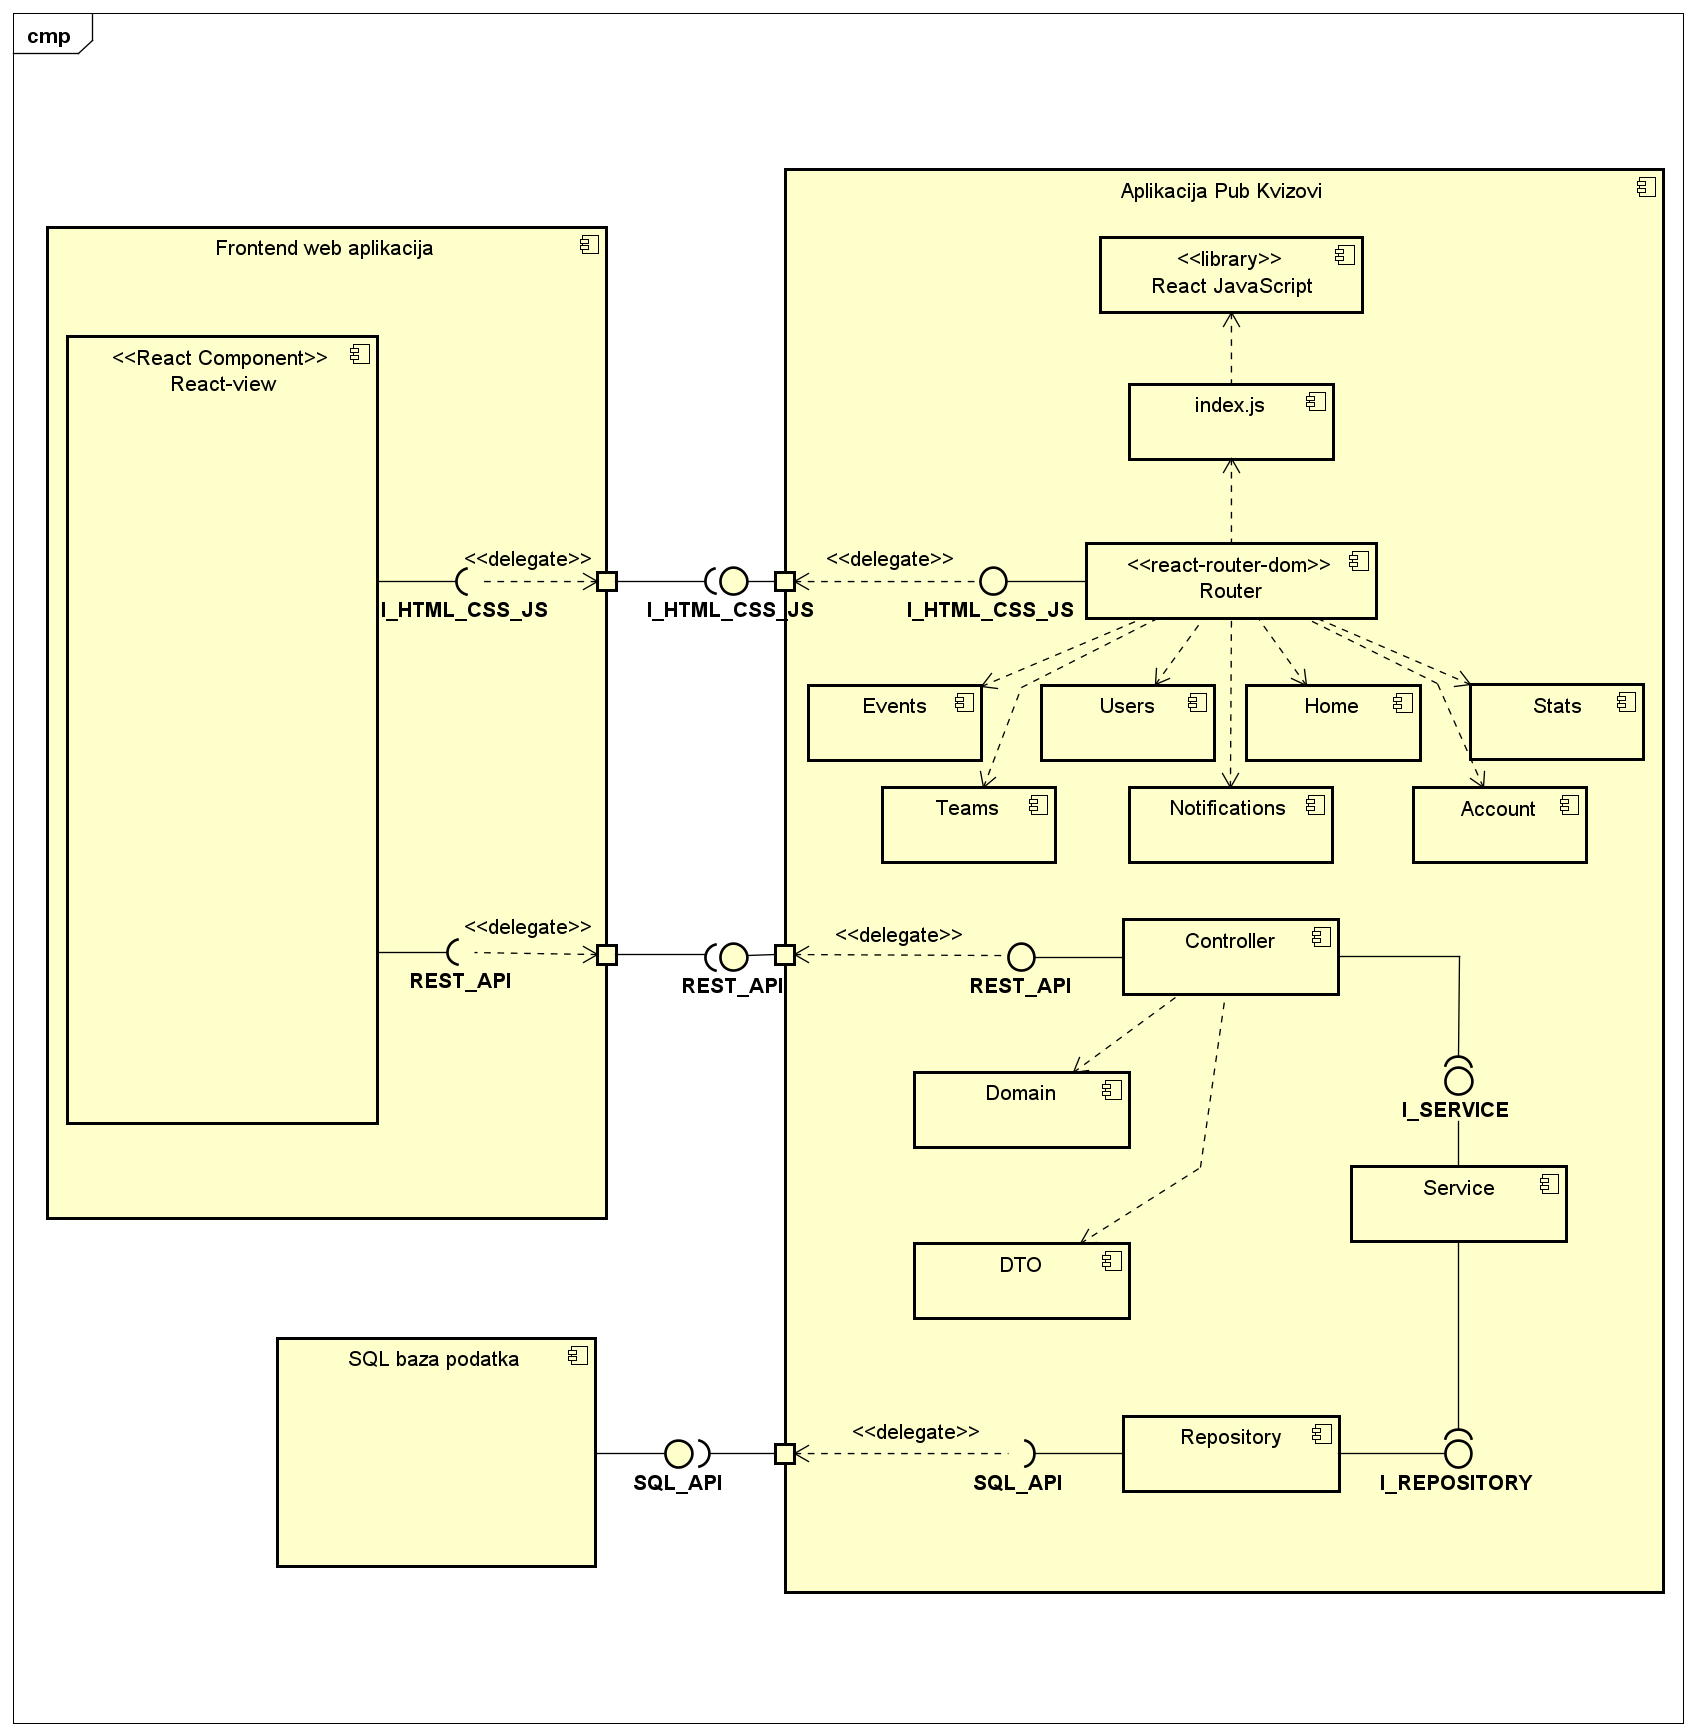
\includegraphics[width=\textwidth]{dijagrami/ComponentDiagram.PNG} 
				\caption{Dijagram komponenti}
				\label{fig:ComponentDiagram}
			\end{figure}
		
	
	\chapter{Implementacija i korisničko sučelje}
		
		
		\section{Korištene tehnologije i alati}
		
			\textbf{\textit{dio 2. revizije}}
			
			 \textit{Detaljno navesti sve tehnologije i alate koji su primijenjeni pri izradi dokumentacije i aplikacije. Ukratko ih opisati, te navesti njihovo značenje i mjesto primjene. Za svaki navedeni alat i tehnologiju je potrebno \textbf{navesti internet poveznicu} gdje se mogu preuzeti ili više saznati o njima}.
			
			
			\eject 
		
	
		\section{Ispitivanje programskog rješenja}
			
			\textbf{\textit{dio 2. revizije}}\\
			
			 \textit{U ovom poglavlju je potrebno opisati provedbu ispitivanja implementiranih funkcionalnosti na razini komponenti i na razini cijelog sustava s prikazom odabranih ispitnih slučajeva. Studenti trebaju ispitati temeljnu funkcionalnost i rubne uvjete.}
	
			
			\subsection{Ispitivanje komponenti}
			\textit{Potrebno je provesti ispitivanje jedinica (engl. unit testing) nad razredima koji implementiraju temeljne funkcionalnosti. Razraditi \textbf{minimalno 6 ispitnih slučajeva} u kojima će se ispitati redovni slučajevi, rubni uvjeti te izazivanje pogreške (engl. exception throwing). Poželjno je stvoriti i ispitni slučaj koji koristi funkcionalnosti koje nisu implementirane. Potrebno je priložiti izvorni kôd svih ispitnih slučajeva te prikaz rezultata izvođenja ispita u razvojnom okruženju (prolaz/pad ispita). }
			
			
			
			\subsection{Ispitivanje sustava}
			
			 \textit{Potrebno je provesti i opisati ispitivanje sustava koristeći radni okvir Selenium\footnote{\url{https://www.seleniumhq.org/}}. Razraditi \textbf{minimalno 4 ispitna slučaja} u kojima će se ispitati redovni slučajevi, rubni uvjeti te poziv funkcionalnosti koja nije implementirana/izaziva pogrešku kako bi se vidjelo na koji način sustav reagira kada nešto nije u potpunosti ostvareno. Ispitni slučaj se treba sastojati od ulaza (npr. korisničko ime i lozinka), očekivanog izlaza ili rezultata, koraka ispitivanja i dobivenog izlaza ili rezultata.\\ }
			 
			 \textit{Izradu ispitnih slučajeva pomoću radnog okvira Selenium moguće je provesti pomoću jednog od sljedeća dva alata:}
			 \begin{itemize}
			 	\item \textit{dodatak za preglednik \textbf{Selenium IDE} - snimanje korisnikovih akcija radi automatskog ponavljanja ispita	}
			 	\item \textit{\textbf{Selenium WebDriver} - podrška za pisanje ispita u jezicima Java, C\#, PHP koristeći posebno programsko sučelje.}
			 \end{itemize}
		 	\textit{Detalji o korištenju alata Selenium bit će prikazani na posebnom predavanju tijekom semestra.}
			
			\eject 
		
		
		\section{Dijagram razmještaja}
			
			\textbf{\textit{dio 2. revizije}}
			
			 \textit{Potrebno je umetnuti \textbf{specifikacijski} dijagram razmještaja i opisati ga. Moguće je umjesto specifikacijskog dijagrama razmještaja umetnuti dijagram razmještaja instanci, pod uvjetom da taj dijagram bolje opisuje neki važniji dio sustava.}
			
			\eject 
		
		\section{Upute za puštanje u pogon}
		
			\textbf{\textit{dio 2. revizije}}\\
		
			 \textit{U ovom poglavlju potrebno je dati upute za puštanje u pogon (engl. deployment) ostvarene aplikacije. Na primjer, za web aplikacije, opisati postupak kojim se od izvornog kôda dolazi do potpuno postavljene baze podataka i poslužitelja koji odgovara na upite korisnika. Za mobilnu aplikaciju, postupak kojim se aplikacija izgradi, te postavi na neku od trgovina. Za stolnu (engl. desktop) aplikaciju, postupak kojim se aplikacija instalira na računalo. Ukoliko mobilne i stolne aplikacije komuniciraju s poslužiteljem i/ili bazom podataka, opisati i postupak njihovog postavljanja. Pri izradi uputa preporučuje se \textbf{naglasiti korake instalacije uporabom natuknica} te koristiti što je više moguće \textbf{slike ekrana} (engl. screenshots) kako bi upute bile jasne i jednostavne za slijediti.}
			
			
			 \textit{Dovršenu aplikaciju potrebno je pokrenuti na javno dostupnom poslužitelju. Studentima se preporuča korištenje neke od sljedećih besplatnih usluga: \href{https://aws.amazon.com/}{Amazon AWS}, \href{https://azure.microsoft.com/en-us/}{Microsoft Azure} ili \href{https://www.heroku.com/}{Heroku}. Mobilne aplikacije trebaju biti objavljene na F-Droid, Google Play ili Amazon App trgovini.}
			
			
			\eject 
	\chapter{Zaključak i budući rad}
		
		\textbf{\textit{dio 2. revizije}}\\
		
		 \textit{U ovom poglavlju potrebno je napisati osvrt na vrijeme izrade projektnog zadatka, koji su tehnički izazovi prepoznati, jesu li riješeni ili kako bi mogli biti riješeni, koja su znanja stečena pri izradi projekta, koja bi znanja bila posebno potrebna za brže i kvalitetnije ostvarenje projekta i koje bi bile perspektive za nastavak rada u projektnoj grupi.}
		
		 \textit{Potrebno je točno popisati funkcionalnosti koje nisu implementirane u ostvarenoj aplikaciji.}
		
		\eject 
	\chapter*{Popis literature}
		\addcontentsline{toc}{chapter}{Popis literature}
		
		
		\begin{enumerate}
			
			
			\item  Programsko inženjerstvo, FER ZEMRIS, \url{http://www.fer.hr/predmet/proinz}
			
			\item  I. Sommerville, "Software engineering", 8th ed, Addison Wesley, 2007.
			
			\item  T.C.Lethbridge, R.Langaniere, "Object-Oriented Software Engineering", 2nd ed. McGraw-Hill, 2005.
			
			\item  I. Marsic, Software engineering book``, Department of Electrical and Computer Engineering, Rutgers University, \url{http://www.ece.rutgers.edu/~marsic/books/SE}
			
			\item  The Unified Modeling Language, \url{https://www.uml-diagrams.org/}
			
			\item  Astah Community, \url{http://astah.net/editions/uml-new}
		\end{enumerate}
		
		 
	
	
	\begingroup
	\renewcommand*\listfigurename{Indeks slika i dijagrama}
	%\renewcommand*\listtablename{Indeks tablica}
	%\let\clearpage\relax
	\listoffigures
	%\vspace{10mm}
	%\listoftables
	\endgroup
	\addcontentsline{toc}{chapter}{Indeks slika i dijagrama}


	
	\eject 
		
	\chapter*{Dodatak: Prikaz aktivnosti grupe}
		\addcontentsline{toc}{chapter}{Dodatak: Prikaz aktivnosti grupe}
		
		\section*{Dnevnik sastajanja}
		
		\textbf{\textit{Kontinuirano osvježavanje}}\\
		
		 \textit{U ovom dijelu potrebno je redovito osvježavati dnevnik sastajanja prema predlošku.}
		
		\begin{packed_enum}
			\item  sastanak
			\item[] \begin{packed_item}
				\item Datum: 12. listopada 2022.
				\item Prisustvovali: svi
				\item Teme sastanka:
				\begin{packed_item}
					\item  upoznavanje
					\item  dogovor oko prijedloga nove teme
				\end{packed_item}
			\end{packed_item}
			
			\item  sastanak
			\item[] \begin{packed_item}
				\item Datum: 20. listopada 2022.
				\item Prisustvovali: svi
				\item Teme sastanka:
				\begin{packed_item}
					\item  sastanak s asistenticom i demonstratorom
					\item  konačan odabir alata i tehnologija
					\item upute o radu
				\end{packed_item}
			\end{packed_item}
		
			\item  sastanak
			\item[] \begin{packed_item}
				\item Datum: 31. listopada 2022.
				\item Prisustvovali: svi
				\item Teme sastanka:
				\begin{packed_item}
					\item  opis teme
					\item  definiranje funkcionalnih zahtjeva
					\item podjela zadataka (obrasci uporabe, opis arhitekture, model baze podataka) 
				\end{packed_item}
			\end{packed_item}
			
			%
			
		\end{packed_enum}
		
		\eject
		\section*{Tablica aktivnosti}
		
			\textbf{\textit{Kontinuirano osvježavanje}}\\
			
			 \textit{Napomena: Doprinose u aktivnostima treba navesti u satima po članovima grupe po aktivnosti.}

			\begin{longtblr}[
					label=none,
				]{
					vlines,hlines,
					width = \textwidth,
					colspec={X[7, l]X[1, c]X[1, c]X[1, c]X[1, c]X[1, c]X[1, c]X[1, c]}, 
					vline{1} = {1}{text=\clap{}},
					hline{1} = {1}{text=\clap{}},
					rowhead = 1,
				} 
				 & \rotatebox{90}{\textbf{Ime Prezime voditelja}} & \rotatebox{90}{\textbf{Ime Prezime }} &	\rotatebox{90}{\textbf{Ime Prezime }} & \rotatebox{90}{\textbf{Ime Prezime }} &	\rotatebox{90}{\textbf{Ime Prezime }} & \rotatebox{90}{\textbf{Ime Prezime }} &	\rotatebox{90}{\textbf{Ime Prezime }} \\  
				Upravljanje projektom 		&  &  &  &  &  &  & \\ 
				Opis projektnog zadatka 	&  &  &  &  &  &  & \\ 
				
				Funkcionalni zahtjevi       &  &  &  &  &  &  &  \\ 
				Opis pojedinih obrazaca 	&  &  &  &  &  &  &  \\ 
				Dijagram obrazaca 			&  &  &  &  &  &  &  \\ 
				Sekvencijski dijagrami 		&  &  &  &  &  &  &  \\ 
				Opis ostalih zahtjeva 		&  &  &  &  &  &  &  \\ 

				Arhitektura i dizajn sustava	 &  &  &  &  &  &  &  \\ 
				Baza podataka				&  &  &  &  &  &  &   \\ 
				Dijagram razreda 			&  &  &  &  &  &  &   \\ 
				Dijagram stanja				&  &  &  &  &  &  &  \\ 
				Dijagram aktivnosti 		&  &  &  &  &  &  &  \\ 
				Dijagram komponenti			&  &  &  &  &  &  &  \\ 
				Korištene tehnologije i alati 		&  &  &  &  &  &  &  \\ 
				Ispitivanje programskog rješenja 	&  &  &  &  &  &  &  \\ 
				Dijagram razmještaja			&  &  &  &  &  &  &  \\ 
				Upute za puštanje u pogon 		&  &  &  &  &  &  &  \\  
				Dnevnik sastajanja 			&  &  &  &  &  &  &  \\ 
				Zaključak i budući rad 		&  &  &  &  &  &  &  \\  
				Popis literature 			&  &  &  &  &  &  &  \\  
				&  &  &  &  &  &  &  \\ \hline 
				\textit{Dodatne stavke kako ste podijelili izradu aplikacije} 			&  &  &  &  &  &  &  \\ 
				\textit{npr. izrada početne stranice} 				&  &  &  &  &  &  &  \\  
				\textit{izrada baze podataka} 		 			&  &  &  &  &  &  & \\  
				\textit{spajanje s bazom podataka} 							&  &  &  &  &  &  &  \\ 
				\textit{back end} 							&  &  &  &  &  &  &  \\  
				 							&  &  &  &  &  &  &\\ 
			\end{longtblr}
					
					
		\eject
		\section*{Dijagrami pregleda promjena}
		
		\textbf{\textit{dio 2. revizije}}\\
		
		\textit{Prenijeti dijagram pregleda promjena nad datotekama projekta. Potrebno je na kraju projekta generirane grafove s gitlaba prenijeti u ovo poglavlje dokumentacije. Dijagrami za vlastiti projekt se mogu preuzeti s gitlab.com stranice, u izborniku Repository, pritiskom na stavku Contributors.}
		
	


\end{document} %naredbe i tekst nakon ove naredbe ne ulaze u izgrađen dokument 


